%%\documentclass[10pt,twocolumn]{puthesis}
%\documentclass[12pt,twocolumn]{report}
%\usepackage[margin=0in]{geometry}
%\usepackage{layout}
%%\documentclass[draft]{york-thesis}
%
%
%%\usepackage{cite}
%%\usepackage[square, comma,sort&compress]{natbib} 
%%\usepackage[numbers, sort&compress]{natbib}
%% \usepackage[pdftex,colorlinks]{hyperref} \AtBeginDvi{\special{pdf:tounicode
%% EUC-UCS2}}
%%\usepackage[top=1in,bottom=1in,left=1.5in,right=1in]{geometry}
%%\usepackage[linesnumbered]{algorithm2e}
%% \usepackage{enumitem}
%\usepackage{kbordermatrix}
%\usepackage{blkarray}
%\usepackage{multirow}
%\usepackage{fancyhdr}
%\usepackage[linesnumbered, algoruled, vlined]{algorithm2e}
%\usepackage{graphicx}
%\usepackage{multicol}
%\usepackage{color}
% %\usepackage{colortbl}
%%\usepackage[table]{xcolor}
%\usepackage{xcolor}
%\usepackage{tabularx}
%\usepackage{alltt}
%\usepackage{array}	
%\usepackage{tabularx}
%\usepackage{verbatim}
%\usepackage{url}
%% \usepackage{subfigure}
%\usepackage{bigdelim}
%\usepackage{bigstrut}
%\usepackage{multirow}
%\usepackage{amssymb}
%\usepackage{amsmath}
%\usepackage{subfig}
%%\usepackage[dvips]{graphicx}
%%\usepackage{amssymb}
%%\usepackage{amsmath}
%%\usepackage[dvips]{graphicx}
%\usepackage{url}
%\usepackage{ctable}
%\usepackage{array}
%%\usepackage{supertabular}
%\usepackage{hhline}
%\usepackage{setspace}
%\usepackage{anysize}
%\usepackage{mathptmx} %math font to times
%\usepackage{makeidx}
%%\usepackage{york-thesis}
%\graphicspath{{./temp/datacenter/}}
%\usepackage{listings,,setspace}
%  \usepackage{courier}
%  
% \lstset{
%         basicstyle=\footnotesize\ttfamily, % Standardschrift
%         %numbers=left,               % Ort der Zeilennummern
%         numberstyle=\tiny,          % Stil der Zeilennummern
%         %stepnumber=2,               % Abstand zwischen den Zeilennummern
%         numbersep=5pt,              % Abstand der Nummern zum Text
%         tabsize=2,                  % Groesse von Tabs
%         extendedchars=true,         %
%         breaklines=true,            % Zeilen werden Umgebrochen
%         keywordstyle=\color{red},
%    		frame=b,         
% %        keywordstyle=[1]\textbf,    % Stil der Keywords
% %        keywordstyle=[2]\textbf,    %
% %        keywordstyle=[3]\textbf,    %
% %        keywordstyle=[4]\textbf,   \sqrt{\sqrt{}} %
%         stringstyle=\color{white}\ttfamily, % Farbe der String
%         showspaces=false,           % Leerzeichen anzeigen ?
%         showtabs=false,             % Tabs anzeigen ?
%         xleftmargin=17pt,
%         framexleftmargin=17pt,
%         framexrightmargin=5pt,
%         framexbottommargin=4pt,
%         %backgroundcolor=\color{lightgray},
%         showstringspaces=false      % Leerzeichen in Strings anzeigen ?        
% }
% \lstloadlanguages{% Check Dokumentation for further languages ...
%         %[Visual]Basic
%         %Pascal
%         %C
%         %C++
%         %XML
%         %HTML
%         Java
% }
%    %\DeclareCaptionFont{blue}{\color{blue}} 
%
%  %\captionsetup[lstlisting]{singlelinecheck=false, labelfont={blue}, textfont={blue}}
%  \usepackage{caption}
%\DeclareCaptionFont{white}{\color{white}}
%\DeclareCaptionFormat{listing}{\colorbox[cmyk]{0.43, 0.35, 0.35,0.01}{\parbox{\textwidth}{\hspace{15pt}#1#2#3}}}
%\captionsetup[lstlisting]{format=listing,labelfont=white,textfont=white, singlelinecheck=false, margin=0pt, font={bf,footnotesize}}
%
%\renewcommand{\rmdefault}{ptm} %for times font
%
%%\setlength{\columnsep}{20pt}
%% \setlength{\columnseprule}{2pt}
%\marginsize{0.75in}{0.75in}{1in}{1in}
% % \doublespacing
%  \singlespacing
%% \oddsidemargin 0.0in 
%% \textwidth 6.5 
% \makeindex 
%
%
%%------
%%\newcommand{\footnoteremember}[2]{
%%  \footnote{#2}
%%  \newcounter{#1}
%%  \setcounter{#1}{\value{footnote}}
%%}
%%\newcommand{\footnoterecall}[1]{
%%  \footnotemark[\value{#1}]
%%}
%%%------
% \makeindex 
% 
%\title{Estimation Chapter}
%% Service  Clouds
%\author{Hamoun Ghanbari}
%% \adviser{My Adviser}
%% \acknowledgements{Thank you very much.}
%% \dedication{To myself.}
%
%
%% \newcommand*{\titleMS}{\begingroup% MS Thesis
%% \drop=0.1\textheight
%% \vspace*{\drop}
%% \centering
%% {\LARGE THE UNIVERSITY}\\[2\baselineskip]
%% {\LARGE\sffamily Conundrums: \\ puzzles for the mind}\par
%% \vfill
%% {\LARGE THESIS}\par
%% \vspace{\drop}
%% {\large some remarks concerning the supervisor \\
%% and the time and place of the examination \\
%% and other administrative details}\par
%% \vfill
%% {\large\bfseries The Candidate}\par 
%% \vspace*{\drop}
%% \endgroup}
%
%%\newcommand{\HRule}{\rule{\linewidth}{0.5mm}}
%% \doublespace 
%\begin{document}
%
% \layout
%\maketitle
% remove up to here 

 \chapter{Models and State Estimstion}
 \label{ch:estimation} 
 
 In this dissertation, models are used to project the behaviour of the system to the future, within the predictive optimization loop.  The modeling enables the autonomic manager to project system's behavior and state under different actions in the future. These models are built on certain elements of well-known theories such as queuing theory. We elaborate on these predictive models in the next chapter. 
However, when working with these type of models, an important task is describing the current state of the system in terms of the model elements.        

  In our case since these models corresponds to the cloud and service instances which run within the cloud, this identification mostly corresponds to estimation 
  of hardware factors (e.g. queue length) or software ones (hardware demand by application) which are treated as hidden parameters of the model
\cite{
rolia_parameter_1995,
rolia_correlating_1998,
courtois_using_2000,
pacifici_cpu_2008,
zhang_regression-based_2007,
zhang_workload_2002,
liu_parameter_2006,
gmach_workload_2007,
gmach_capacity_2007}. 
%
For example, measuring service times or demands for each service instance, even if technologically possible, is not practical because of the overhead introduced. 

The objective of an estimator is to describe the system (or environment) in terms of a given parametric model. 
This identification process includes finding or estimating parameters of the model using the data obtained from the system (or environment) in in ongoing fashion.  

In the remainder of this chapter we describe our approach for parameter estimation and tracking in section \ref{sec:dynamic-classification-and-estimation}. The applicability of the proposed approach is demonstrated by the experiments in Section \ref{sec:experiments}. Related work, conclusions, and future works are discussed in Sections \ref{sec:related-work} and \ref{sec:conclusions-and-future-work} respectively. 

\section{Problem}
Assume the datacenter is composed of a set of $n$ physical machines (PM)s represented by the set $P={p_0,...,p_n}$. 
 Moreover, consider $m$ web based transactional applications \texttt{$app_1$},..., \texttt{$app_m$} are deployed on the cloud while each application runs within one or more VMs and experiences a particular workload.  
To simplify the example we model all deployed applications  
as a single workload on the whole infrastructure. 
In other words we aggregate the effect of applications on each physical machine. 

Typically, the data available from each $k$'th PM includes:  
 \begin{itemize}
\item  $R_k$, the mean total delay per user request, assumed to include queuing and service,
\item  $U_k$, the mean utilization 
\item  $Q_k$ the mean queue length  
\end{itemize}
Here the utilizations and queue length are associated with the dominant resource such as CPU, but in case applications stress two or more resources, each can be treated individually. However, response time is a higher level end-to-end metric and includes the aggregate delay for all resources the request been through in a PM.   % and usually obtained at server OS process level     

Also, the overall system throughput can be obtained by monitoring the number of transactions processed by one of the servers over a time interval % [im not sure if throughput can be measured separately, i think it should because these servers run in parallel].
 [ Also, the throughput (or service rate?no) in each server can be obtained by monitoring the number of transactions processed by the server over a time interval.]  
 \begin{itemize}
\item  $X$, the throughput of requests from Users, per second. 
\end{itemize}

% the thing is that service rate is natural capability  of the server or does it depend on the number of request that are actually coming to a server, so what is measured is not reallyt what server can do but a equilibrium of server and other servers

 % Note that in a stable queuing network, throughput is obtained as whole and is uniform within all nodes in the network, which again I'm not sure 

% \footnote{the effect of adding server in homogenous cluster is discussed in subsection ... but the effect of slow node in the cluster depends on the load balancer policy, maybe it reduces the service rate to the slowest node service rate or maybe it just has a linear contributing factor to the service rate. Actually we can have a section in which we disscuss nested or layered models in which the service rate itself deepnds on other things, and is involved in the equations (like the menace example and the dynamic model), and is not like fixed demand. because service rate which involves other things might be needed to be tracked in a different way than demand/} I think this throughput limiting effect of server-load balancer can be described by nested service rate oriented models. lets see how they track service rate? do they just say, o a new server is  just going to change the service rate of the cluster? 
%doesn't matter if the server is heterogeneous and this rate is tracked like we don't know how its changing. 
%
%So in the forward projection model each node in the queuing network should correspond to a service like DB because by adding and removing servers we are trying to say that although the applicantion now has demand on the added servers, but the traffic is splitted (and we don't know how its splitted), so why not tracking the service rate or throughout of the whole cluster for 
%the app and the forward model ....
%well the cluster throughput depends on each node's response time which in turn depends on the queue length on the node which is affected by the splitting of traffic. 
%
%maybe we should work on m-server model, more. 
%
% and its service rate should be tracked and projected to future 
% the difference between arrival rate and system throughput (or service rate (although in stable state they are equal) forms the transient behaviour of the system. 

Also in case the deployment is tired, response time metrics could be gathered about overall
delay in all tiers rather than one tier: 
 \begin{itemize} 
\item  $R$ the mean time for a user to cycle through one response % $N=XR$,
\end{itemize}
Assume all the information captured from the real system, is summarized in a measurement vector $z$.

Based on the specific situation, a subset of the metrics from a subset of servers might be missing. 
For example in perfect information case one can have 
% Here we enumerate several example forms that missing data scenario could take:
response times, utilization measures, and system throughout: $z=[R_1, ..., R_n, X]$. 
It is possible that the monitoring framework does not supply a specific measurement such as server utilizations:  $z=[R_1, ..., R_n, X]$.  
It is also possible that some part of data from the monitored servers is missing,
 for example $z=[R_1,...,R_{n'}, U_1,...,U_{n''},X], n' < n, n''<n$. Or sometimes both cases happen, for example when some utilization measures, and system throughout are available: for example $z=[U_1,...,U_{n'}, X], n'<n$.
  
  In all these cases, the entities to be estimated are those where causal relationships originating from. 
  which include service demands or their subset,  and the workload component, which is the number of users in the system and think time in closed case and the arrival rate in the open case, for example 
 $ x=[D_1, ..., D_n] $.   
  Note that if the entities with root of causal relationship, if not tracked, should be inserted in the models. These include number of users ($N$), think time ($Z$), and server multiplicity.  
  % the kalman filter part we should have an example how this thing is done
  
%  $H$ will be:
% .......
% 
%case 8:
%The model was set up for a fixed number of seven users, while the actual system (as in Case A1) has $N = 4$. $N$ is not tracked and thus is not corrected. (meaning that state vector $x$ does not include $N$). basically everything that needs to be corrected should be put in $x$, and it should somehow get delated to observations.  

%
%\subsection{Performance Models and Causal Relationships} 
%N, Z, D-> X, R
%X,D->R 
%
%% Derivatives of h with respect to N , D
% % in this case the input is N, the output is R and U and/or X, and 
% % throughput is the latent variables  
% 
%In all examples, there are fixed parameter values that are not tracked, and are just inserted in the models, such as number of users $N=4$, and , think time $Z=0$, and servers have multiplicity of $m_i= 1$.
% 
%  
% 
%\subsubsection{The Workload component}
%%Load intensity of transactional systems 
%%From modeling point of view, service instances are usually parametrized by hardware demand per request and the traffic or workload.  
%%% The major performance characteristics for transactional applications are average response time ($R$) and throughput ($X$). 
%  Essential to the modelling approach is the workflow component.
%   Workloads can be  as viewed in different layers.  at hardware layer the workload is a number of CPU cycles used for 2nd, the amount of memory  used,  reads and writes on disk,  and the network interface access
%   done by the corresponding processes or operating system.
%   However, the  abstraction level workload is modelled in this thesis is higher.
%    workload is modelled in application level,  where the application is  either transactional, or batch type. 
%     We model the traffic of transactional application  either as {\it open} or {\it closed}  pool of customers.  
% For web applications customers  correspond to web requests. 
%In open mode, customers are assumed to make requests on average every $\tau$ seconds, independent of when they receive responses for previous requests. Open workloads are identified
% by request inter-arrival time ($\tau$) which is measured in seconds or arrival rate ($\lambda$) which is  measured in requests per seconds.  As in the literature, we assume that the arrival rate ($\lambda $) is a homogeneous Poisson process, and that inter-arrival times ($\tau $) are exponentially distributed with parameter $\lambda $ (mean of 1/$\lambda $).
%% Using mean value analysis, one could derive a solution for general open queuing network models \cite{lazowska_quantitative_1984}.  
%In case of open multi-class models where there are $C$ customer classes, workload intensity is denoted by $\lambda\equiv(\lambda_1 \dots \lambda_C)$, where $\lambda_c$, is the class $c$ arrival rate.
%
%% We briefly mentioned the algorithm together with set of equations forming this model in 
%
%In a closed transactional model, clients are assumed to wait for responses to their requests.  Upon receipt of this response, a client spends time analyzing (i.e., determining the next action to take) before issuing a further request. Closed models are defined by the number of users ($N$) and think time ($Z$). 
% A closed multi-class model consists of $C$ classes, each of which has a fixed population. We denote the workload intensity by $N\equiv(N_1 \dots N_C)$, where $N_c$, is the class $c$ population size. Obtaining solutions for closed models is somewhat more complicated than for open models and usually involves iterative methods with some convergence criterion. 
%
%% \textbf{Batch Workloads}, in contrast to transactional ones, are usually quantified by long-running jobs instead of short term requests. As a result, the traffic in batch workloads can be highly irregular, to the point that measures like request rate would become meaningless.  In extreme cases, one massive job (e.g. a peta-byte sort) can take a whole cluster of worker instances. In this case, one should model the system on per-request basis.   Moreover in grid environment, there is a lot of variation is resource usage, making it hard to perform resource-to-performance mapping. Variations are due to, tasks hugging resources (e.g. CPU, disk, or network) for a while and causing them to reach 100\% utilization; then releasing the resources after they are terminated and making utilizations suddenly drop.
%
%% batch workload is a pure pull based (pull on data or code)
%% it usually gets a cpu, network or disks t o 100% utilization, since the system pulls as much as it can. and has intervals of freeness 
%% from queuing theory based modeling perspective it is special case of closed queuing network with zero think time
%% however it is actually harder than that because jobs are splited into tasks, jobs run in parallel, and jobs are different in nature (like cpu intensive and disk intensive) 
%% with distributed file system, disk and network are interchangeable
%
% the 2nd feature of the workload when viewed in this perspective, is the resource demand it  imposes on each resource of the system for each request. Meaning that each request is going to  consume certain amount of CPU cycles, disk  reads/writes, network interface interaction.
%  resource demand is denoted as a vector of stealer values where each value represents the demand on a separate resource when there are multiple classes of users. each classas a result.is going to have its own demand on each resource.  the demands Armando by inmate treats
%
%From modeling point of view, applications are usually parametrized by hardware demand per request and the traffic or workload.  
%
%% state space form ....

%\subsection{Estimation through regression} 
%
%There are different approaches to estimate hidden parameters of a given performance model using the measured data. 
%
%As far as we have seen in the literature, there are two major techniques to discover these parameters.
%The first approach is to select some equations of the performance model and reshape them into 
%a commonly known parametric form in which un-accessible variables are mapped to model parameters
%and the training dataset provides value for all inputs of outputs of the model (i.e. no missing data). 
%In this case common supervised learning methods such as regression techniques can be used to estimate unknown parameters
%
%optimization form of solving, and comparison to regression technique 

%Idea of state
%x(t) is called state of system at time t since:
%� future output depends only on current state and future input
%� future output depends on past input only through current state
%� state summarizes e?ect of past inputs on future output
%� state is bridge between past inputs and future outputs

\subsection{Conventional Methods}       
In frequentist statistical theory, the estimation is usually carried out using Maximum Likelihood Estimation (MLE) or as a special case Least Square Estimation (LSE). In MLE, one tries to choose a distribution that maximizes the likelihood of observed data, (i.e. $max P(data|model)$).
This distributions are usually either continuous and parametarized or with a finite set domain. 

One of the easiest methods in performance estimation area (used for example in  \cite{pacifici_cpu_2008})  is using LSE on the linear relation between a server utilization measurement and the arrival rate of customer classes in open queuing networks:     
\[ U_k=\sum_{c=1,...,C} \lambda_{c} D_{c,k} \]
here $U_k$ denotes utilization of resource centre $k$, $\lambda_c$ denotes the workload component of customer class $c$, 
 and $D_{c,k}$ denotes class $c$ service demands on $k$'th resource center. 
 When a queuing centre is monitored for a time interval of length $T$, 
 there will be $T$ measurements:
 \[ {U_{k}}_i = \lambda_{i}^T D_k + v_i,\  i=1,...,T \]  
here $\lambda$ was considered a vector of arrival rate for all classes:
\[ \lambda_i^T=[\lambda_1, \lambda_2, ..., \lambda_C] \]
 Lets assume $v_i$ is an IID noise with density $p(z)$,
 then MLE estimate of $D_k$ would be the solution to: 
 \[ \text{maximize } l(D_k)=\sum_{i=1}^{T} \text{log } p({U_{k}}_i -  \lambda_i^T D_k)\]
 if the noise $p(z)$ is gaussian (i.e. $N(0, \sigma^2)$), then 
  ML estimate is LS solution, thus the problem reduces to:
\[\text{minimize} \sum_{i=1}^{T}({U_{k}}_i -  \lambda_i^T D_k)^2  \]
  Thus the solution for all centres can be obtained by: 
 \[ D =  ( \lambda^T \lambda)^{-1} \lambda^T U \] 
 \footnote{If $\text{rank } A=n$.} 
%% \footnote{Note that the service demand of a class of service on a processing center is the total time the processing center spends for each request (or client) of that class of service.} 
% The model in a linear matrix form is as follows:
% \[ U=\lambda D + \epsilon \]
%% where 
%%, to form a multivariate linear regression problem with $C$ independent variables:  $Y = X\beta + \epsilon$. 
 here $U$ is a $T\times K$ matrix of resource utilization samples over time $T$, $\lambda$ is $T\times C$ matrix of arrival rates sampled over the same interval, and $D$ is $C\times K$ matrix of resource demands for all classes of service on all resources. %, and $\epsilon$ is ransdom term with gaussian distribution. 
% The matrix of user demands $D$ in this case can be found through simple equation:

The problem with the above approach is that, it cannot take into account other measurements from system that are related to demands in non-linear fashion.  
Other examples of CPU demand estimation using regression analysis are \cite{rolia_parameter_1995,zhang_regression-based_2007,rolia_correlating_1998}.
In many cases, specially when complex performance models are used, the possibility of finding a parametric form whose corresponding MLE, has a convex form is very low. When the solution of the model is described in terms of numerical methods instead of parametric form, nonlinear least squares or regression algorithms such as Levenberg-Marquardt \cite{wild_nonlinear_2003} or \cite{dumouchel1989integrating} can be used to find the model parameters. In \cite{dumouchel1989integrating}, for example,  a weighted nonlinear regression is iteratively refited. Weights at each iteration are based on each observation's residual from the previous iteration. Points that are outliers are downweighted and their influence on the fit is decreased. Iterations continue until the weights converge.
Note that the convergence of the parameters in this case 
and the correctness of estimation depends on the underlying model. 
If applying the MLE on the model does not follow a convex form, it is quiet possible that the regression does not converge or converges to a wrong value.   

As examples of works using these techniques are 
\cite{courtois_using_2000} where regression splines are utilized. 
%instead of linear and polynomial regression functions.  
 In \cite{zhang_workload_2002} and \cite{liu_parameter_2006}, multi-class queuing models were used to infer the per-class service times at different servers of a two-tier web cluster using throughput, utilization, and per-class response time measurements. 
They try to minimize the sum of predicted response time mean square errors using a non-linear optimization solvers and quadratic minimization programs. In addition, MLE together with queuing model have been used for the same purpose \cite{kraft_estimating_2009}.

\subsection{Solution through Bayesian Estimation}  
Another set of proposals adopted by \cite{woodside_use_2005,xu_performance_2005,zheng_tracking_2005}
use the Bayesian statistics approach for performance estimation problem. 
 %to track unknown parameters of performance model. 

In the Bayesian approach, probability estimate for a hypothesis is updated as additional evidence is learned; this makes it a good fit for estimation tasks on sequential data. One can look at performance data as a sequence of measurements,  where the unknown performance parameters are changing parameters to be estimated from observations. 
To perform estimation of this kind, there is a need for a \textit{state-space model} that specifies the dynamic and measurement relations among latent states and observations. 

% \cite{xu_performance_2005,zheng_tracking_2005}
%In tracking filter approach, the performance metrics of the system are treated as  sequential data. An state-space model is utilized within the tracking filter.  

% One of the benefits of this approach is the fact that we can specify dynamics of the state transition explicitly. 
%++
The elements specified in the model are: 
% Q: a finite set of N states  Q = {q0, q1, q2, q3, ...}
(i) A domain of possible states,
% An explicit start state q0 or alternatively,
%a prior distribution over start states: {�1, �2, �3, ...}, ? �i = 1  The set of final states: qF  
(ii) an explicit initial state or alternatively, a prior distribution over start states,  
% N ? N Transition probability matrix
(iii) the state transition equation, and 
% N ? |V| Emission probability matrix
(iv) the state-output or observation equation. 
% Sequence of observations O = o1, o2, ... oT
% Likelihood: Given an HMM ? = (A, B, �), and a sequence of observed events O, find P(O|?)
% Likelihood: 
% Given a model ? including state transition equation, state output equation, initial states, and a sequence of observed events O, find $P(O|?)$
%
% In this case, observable portion of data is mapped to input or output variables while states (i.e. latent variables) are hidden.  

%  variables can be divided as input, state, and output (as opposed to input and output). Output variables depend on inputs as well as states.

% param�tre estimation versus state-estimation 
The hidden portion of data to be estimated is associated with state variables (rather than output variables). Observable portion of data is divided into dependent and independent variables (input and output). 
Lets assume $x$ ($x_k \in \mathtt{R}^n$) represents the performance model parameters and $z$ represents the measurement vector. 
For estimation, an equation in state space form is used to relate $x$ to $z$ which in non-linear case has the form:
 \[ x_{k + 1} = f(x_k, u_k)+G(x_k,u_k)w_k \]
 \[ z_k = h(x_k)+v_k \]  
 where 
 $f$ determines the state transition, 
 $h$ determines the observation, 
 $k$ denotes the descrete time, $u$ represents a known vector (or system input), 
 $w_k$ is process noise with normal distribution, zero mean, covariance of $Q_k$: $N(0,Q_k)$,  
 $v_k$ is observation noise with normal distribution, zero mean, and covariance of $R_k$: $N(0,R_k)$, and $G(x_k, u_k)$ represents the noise structure and yields a matrix with full column rank. 
 
 Parameters of the model to be estimated are  
 noise structure, the model parameters and the state and measurement noise covariance structures.
 \footnote{Note that, determining the optimal parameter estimates 
 cannot be done using a weighted least squares optimization of the measurement residuals (i.e. $y_k - h(x_k)$) with respect to the model parameters $\theta$, since the process of the model is non-deterministic.}
 
 % determining the optimal parameter estimates corresponds to a weighted least squares op- timization of the measurement residuals (i.e. yk ? h(xk)) with respect to the model parameters ?.
 
Having this model and an observation sequence, one can find the most likely (hidden) state sequence. This state sequence estimate
is the one that maximizes the likelihood (probability) of the observed data given the model:
\[ x^+_T=arg max_{x_T} p(x_T|y_0,...,y_T) \] 

In bayesian form the estimator performs an update on state estimates, based on the information up to the current time point, in a way that this long-term likelihood of the observations is maximized:
 Ideally, state estimators should solve the problem
%\[ x_T+ = arg max_{x_T) p(xT|y0,...,yT) \]
%xT
%in which p(xT|y0,...,yT) is the probability that the state of the system is x_T givenmea- surements y0, . . . , yT . Equation (3) is referred to as the maximum likelihood estimate. In the special case that the system is not constrained and in equation (2)
 \begin{equation}\label{e:barwq}\begin{split}
& max_{x_0,...,x_T} p(x_0,...,x_T|y_0,...,y_T)= \\
 &min_{x_0,...,x_T} -log p(x_0,...,x_T|y_0,...,y_T)= \\
& min -log p(x_0) - \sum_{k=T-N+1}^{T-1} log p(x_{k+1}|x_k) - \\
 &  \sum_{k=T-N+1}^{T-1} log p(y_k|x_k)\\
 \end{split}\end{equation}  
This gives rise to a least-squares optimization:
  \begin{flalign*}
 \text{minimize}_{x_0,...,x_T}  \  &  (x_0 - \hat{x}_0)^T \Pi^{-1}(x_0 - \hat{x}_0)+ \\ 
 & \sum_{k=0}^{T-1} w^T_k Q^{-1}_k w_k + \\
  & \sum_{k=0}^{T-1}  v^T_k R^{-1}_k v_k  \\ % \sum^{N'-1}_{k=0}
 \text{subject to:}  \\ 
 & x_{k + 1} = f(x_k, u_k)+G(x_k,u_k)w_k \\
 & z_k = h(x_k)+v_k 
 \end{flalign*}
 
% \begin{equation}\label{e:barwq}\begin{split}
%   min & (x_0 - \hat{x}_0)^T \Pi^{-1}(x_0 - \hat{x}_0)+ 
% \sum_{k=0}^{T-1} w^T_k Q^{-1}_k w_k + \\
%  & \sum_{k=0}^{T-1}  v^T_k R^{-1}_k v_k \\
%   
%  
%
%\end{split}\end{equation}  

  
% This update rule gives the most likely current states of a system in each step. 
% The estimator tracks the ongoing (i.e., online) changes in latent variables.

For linear systems, that have the certain properties, there is a closed form step-by-step solution to this optimization well-known as Kalman filter. 
The properties are as follows: (i) $F(x_k,u_k)$ is linear with respect to $x_k$, (ii) $h(x_k)$ is linear with respect to $x_k$, and (iii) $G(x_k, u_k)$ is a constant matrix, and (iv) all latent and observed variables have Gaussian distributions. Such model is denoted by:
\begin{equation}\label{e:barwq}\begin{split}
 x_{k+1}&=A_k x_k+B_ku_k+w_k \\ 
 z_k &= H_k x_k + v_k 
 \end{split}\end{equation}  

For cases where observation equation is non-linear such as:
\[ z_k = h_k(x_k) + v_k \]
extensions have been proposed to KF. Extended Kalman Filter (EKF) is one such approximation, where  nonlinear system is linearized, then Kalman filter (the optimal, unconstrained, linear state estimator) is applied to obtain the state estimates. 

In the next subsection, we elaborate on the  the estimation processes of EKF, while in the subsequent subsection we describe
the process and observation model used for estimation. 

%Sequential least-squares approach for estimating...
% (Dolan & P. C. M. Molenaar, 1991; J. H. Oud, van den Bercken, & Essers,1990; Zarchan & Muso�, 2000) is one of the earliest used....
%
%actor scores are estimated by minimizing prediction errors in the least squares sense. 
% 
%In other instances, the KF is often used in conjunction with a maximum likelihood procedure termed prediction error decomposition to estimate
%parameters for dynamic and time series models (Durbin & Koopman, 2001; Kim & Nelson,1999; Shumway & Sto�er, 2004). 





 % \cite{tanizaki_nonlinear_1996,wan_unscented_2000,welch_introduction_1995} 

%
% \subsubsection{Solution to Flat Models}
%\label{sec:solution-flat-model}
%Separable flat queuing network models (as opposed to layered, tiered, etc) are usually a simplistic yet fine approximation of how system is performing at hardware layer.
%Devices can be mapped to queuing centers and requests can be mapped to customers.
%General mean value analysis (MVA) based solution for flat queuing network models can be obtained easily based on a set of laws governing these networks.

%\subsection{Modeling performance metrics of Applications}  
%
%%\subsubsection{steady-state models}  
%% A non-linear model derived from the mean value based formula for open queuing networks ($R=D/(1-\lambda D)$) \cite{lazowska_quantitative_1984} extended 
%%to account for capacity ($D_j=\frac{\beta_1 d_j}{\gamma_j-\beta_2 d_j/{\tau}_j}$) 
%%%which estimates the average response time per request ($R$), based on the requests arrival rate ($\lambda$)
%%% and per-request server demand ($D$) \footnote{Server demand is the amount of time each request will spend in the queuing center to be processed.}.
%%This equation can be derived by substituting $D_j$ with
%%  $d_j/\gamma_j$ and ${\lambda}_j$ with $1/{\tau}_j$ from the base
%%  formula, and adding model coefficients (i.e. $\beta_1$ and
%%  $\beta_2$) to compensate for the differences between the system and
%%  pure queuing model. The substitution requires the arrival rate
%%  ($\lambda $) to be a homogeneous Poisson process, and inter-arrival
%%  times ($\tau $) to be exponentially distributed with parameter
%%  $\lambda $ (mean 1/$\lambda $).        
%%  
%%\subsection{Model} 
%%\label{sec:model}
%In order to capture the behavior of multi-tier web services deployed in a data center environment we used Layered Queuing Model (LQM). In LQM, a web application is viewed as layers of software introduced by the different tiers (e.g. web and database servers) and hardware layers of the underlying infrastructure. Each layer is represented by a Queuing Network Model (QNM) which can be solved by the mean value analysis. 
%
%
%Model inputs for LQMs include 1) the structure of the model including the services and their interactions for representative scenarios, and a topology of the underlying middleware and hardware and 2) the quantitative performance metrics such as workload component ($W_i$), identified with the number of users ($N_c$) and mean think time ($Z_c$) for close models or by the external arrival rate (${\lambda }_i$), and service times or demands ($D_c$) for each class of service $c$. Outputs of LQM include response times ($R_c$), throughput ($X_c$) for each class and server utilization ($U_j$) for each server.
%
%We assume that there are $C$ classes of requests; the ``User'' block in Figure 3 represents $N_c$ users in class $c$ at their browsers. We use $Z_c$ to denote the mean think time of class c users. $N_c$ and $Z_c$ are the workload parameters for class $c$; they correspond to the $W_i$'s defined earlier. 
%
%Variation in load arriving at the system can be modeled by variations in $Z_c$ or in $N_c$; a larger $N_c$ or a smaller $Z_c$ leads to a higher level of offered load.
%
%\begin{figure}[h]
%	\centering		
%	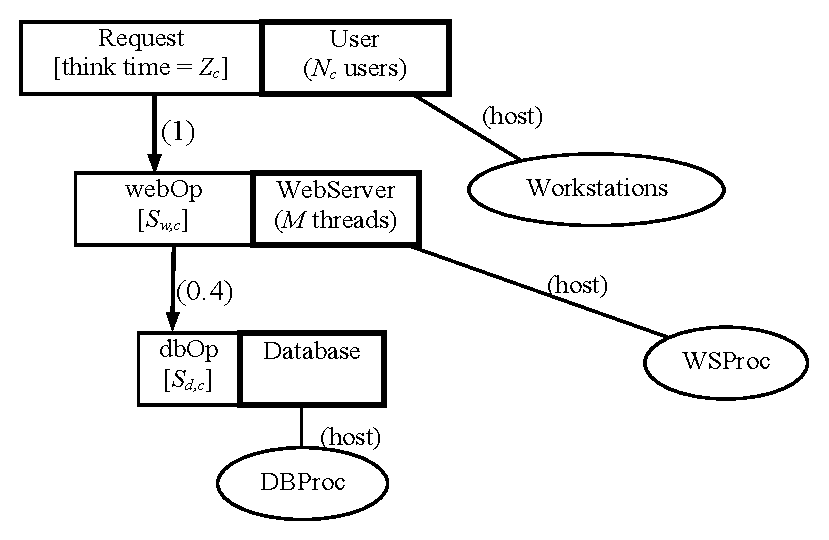
\includegraphics[width=0.45\textwidth]{image/image-LQM-structure.eps} 
%	\caption{Multiclass Layered Queuing Model of a Web application.} 
%	\label{fig:fig3}
%\end{figure}
%
%Figure 3 shows a typical Layered Queuing Model (LQM) of a web-based application. 
%
%The ``WebServer'' block represents the server software with $M$ threads, running on processor WSProc (this is indicated by the ``host'' relationship). The box labeled ``webOp'' represents the operation done for the users, and requires a mean CPU demand of $D_{w,c}$ for requests in class c and on average 1 database operations. The database is running on its own device DBProc. ``dbOp'' represents the mean CPU demands of $D_{d,c}$ at DBProc for a class $c$ request.
%
%Outputs of LQM of Figure 3 include:
%
%\begin{itemize}
%\item  $R_c$ -- mean response times to class c users ($R_1,\dots ,R_C$)
%\item  $R^d_c$ -- mean response times to class c users at database server ($R^d_1,\dots ,R^d_C$)
%\item  $X_c$ -- throughput of class $c$ ($X_1,\dots ,X_C$)
%\item  $U_w$ -- utilization of web server processor
%\item  $U_d$ -- utilization of database processor
%\end{itemize}
%
%Usually, the directly measurable performance data are those given by model outputs, averaged over a measurement time interval of length $T$: \[z=[R_1,\dots,R_C, R^d_1,\dots,R^d_C, X_1,\dots,X_C, U_w,U_b]\]
%Values for the think time $Z_c$ and the CPU demands $D_{w,c}$ and $D_{d,c}$ are not directly accessible at run time. They also vary over time, so we compute and track them indirectly by using the Extended Kalman filter based on the available measured data (See next section).



\subsection{Estimation through tracking filters} 
% \subsection{Extended Kalman Filter Estimator} 
 
In this subsection, we describe an extended Kalman filter [19],[20] (which is a variant of the Kalman filter [24]) to be used by the �State Estimator� to estimate model states and parameters based on the available measured data. Figure 2 depicts the architecture of this extended Kalman filter. Let $x$ and $z$ be vectors representing the parameters and measured performance, respectively. The model maps $x$ to an output vector $y$ (i.e., $y=h(x)$) which represents the predicted performance. The filter then estimates $x$ (which is not directly measurable) based on the observed performance $z$. 

Assume, the matrix $H_k$ is the matrix of partial derivatives of the model function $h$, with respect to the parameters at their current values $x_{k-1}$. Thus, $H_k$ is a matrix of sensitivity values for h.


Assumed prior knowledge of the filter includes distribution of initial state, and process and measurement noise structures: 
\begin{equation}\label{e:barwq}\begin{split}
  x_0  \\
  P_0&=E[(x-\hat{x}_0)(x-\hat{x}_0)^T]  \\
  Q_k &= E[w_k w_k^T]  \\
  V_k &= E[v_k v_k^T]  \\ 
 \end{split}\end{equation}   
 where
   $x_0$ is initial estimate,
    $P_0$ is initial error covariance matrix  \footnote{Note that with the assumption that $x$ has multi-variate gaussian distribution, at any given point in time $\hat{x}_k$ and $P_k$ fully present the state vector distribution. This also applies to $\hat{x}_0$ and $P_0$.}, and 
   $Q$ and $V$ are the covariance matrices for $x$ and $z$, respectively.
  
The filter computations are recursive, beginning from an initial estimate $x_0$, and an initial error covariance matrix $P_0$. Each recursive step and can be summarized as follows:

\begin{enumerate}
\item 
 the �Kalman Gain� matrix $K_k$ is computed as follows:  
\[K_k  =P_k^- H_k^T (H_k P_k^- H_k^T+ V_k )^{-1} \] 		

The core filter calculation is the update of the state estimate $\hat{x}_k$ and covariance error estimate $P_k$ by the linear feedback equation:
% \[x_k   = x_{k-1}  + K_k  e_k\]		
\[e_k   = z_k  - h(x_{k-1})\]
\[ \hat{x}_k = \hat{x}_k + K_k e_k \] 
\[ P_k=P_k^- - K_k H_k P_k^-   \]
here $e_k$ denotes the prediction error vector obtained from the current modelled and observed output vectors ($h(x_{k-1})$ and $z_k$ respectively), and $P_k^- $ denotes value of $P_k$  at time $k$ given measurements up to time $k-1$ (i.e. $P_{k|k-1}$). 
 	
\item 
 it projects state estimate $\hat{x}_k$ and error covariance matrix $P_k$ forwards one step:  
\[ \hat{x}_{k+1} = F(\hat{x}_k,u_k) \] 
\[ P_{k+1}^-  = AP_kA^T+Q \]	
\end{enumerate}

The optimality and convergence properties of the Kalman filter depend on the way the functions are linearized around the current estimate of x. 
 This Extended Kalman filter (EKF) [25] linearizes $h(x)$ by a first order Taylor series around the state estimate and does not take linearization errors into account. Other variants of the filter, like the Unscented Kalman filter [26] or the Divided Difference filter [27] capture the linearization errors in the covariance matrices. They were shown to provide better estimates when dealing with non-linear changes of x, while EKF provides better performance when dealing with non-linear $h(x)$.
 
 \begin{figure}[h]
	\centering		
	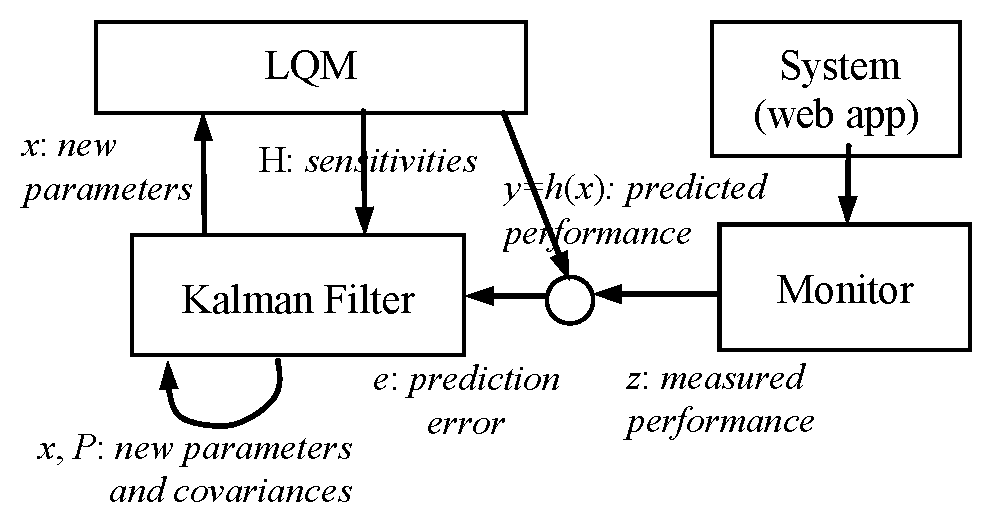
\includegraphics[width=0.45\textwidth]{image/image-tracking-structure.eps}  
	\caption{Kalman filter architecture.} 
	\label{fig:fig4}
\end{figure}

\section{Process Model}   
% its either about demand or service rate 

\subsection{Random Walk} 
 The first process model that can be chosen to describe the system is "Random Walk".  In this scheme the system state  $x_k$ (here demand and workload) is assumed to evolve under random walk and due to a random drift $w$:
\[ x_{k+1}= x_k+ w_k \]
% short form for $x_{k+1}(i) = x_k(i) + w_k(i)$ 
 This means that minimal assumption is made during estimation of hidden parameters of this model: that the covariance matrix for $w_k$ is known (we denote it by $Q_k$). 
 Usually the covariance matrix is diagonal since workload components (number of users and think time) and user demands are assumed to change independently. The values are sometimes set according to 
 \[ Q_{i,i} = \alpha  x_0(i) \]  
where $x_0(i)$ is the initial value of the $i$-th state variable to be estimated,  
 and $\alpha$ is the ratio of expected changes for $x_i$'s,  % usually set around 0.02
 with respect to initial values of them.   
 %  Various values of Qfac were used to evaluate their impact.
  
\subsection{Autonomous Linear Dynamics}
Random walk model, because of minimal configuration needed, is practical and roboust for being used in an estimator. This model however, due to minimal assumption,  is unable to explain \textit{trends} in state variables and thus one cannot use it for prediction:
  \[ \hat{x}(k+j|k) = \hat{x}(k) \]
 

 making $A_k = \mathtt{I}$

\subsection{Higher Order Dynamics} 
In order to model trends
the random walk model would certainly fail. 
Even a first order vector, linear, difference equation of the form $x_k=A x_{k+1}+w_k$ might not give good estimation results. This is sometimes because, first order difference equation might not be able to capture the variables trends.  
For example in case parameter values change with sinusoidal patterns 
the second order model provides better performance during estimation [...] because a sinusoid is exactly second order in dynamics: $y''=Ay$. 
 
In higher order model next value of parameters depends not just on the current value, but on the previous one as well. Here such $\mu$'th order linear dynamical system is presented: 
\begin{equation}\label{e:barwq}\begin{split}
x_{k+1} & = A_{1}x_{k} +...+A_{\mu} x_{k-\mu+1} \\ 
x & \in \mathbb{R}^n , A:\mathbb{R}^n \rightarrow \mathbb{R}^n 
 \end{split}\end{equation}    
  we can reduce this equation to first order state-space form by first defining the state variables as stack of the parameter values  of the past $k-1$ intervals:   
\[
 z = \begin{bmatrix}
       x_{k} \\
       x_{k-1} \\
       \vdots \\
       x_{k-\mu+1} \\
     \end{bmatrix}
     \in R^{n\mu}
\] 
and then using a $\mu n$-by-$\mu n$ block companion matrix (lets denote it by $F$) to down shift the state vector and pad it with a linear combination of elements from original higher-order model: 
\[
z_{k+1}=
 \begin{bmatrix}
%       A_1(z_k) & A_2(z_k) &  \hdots & A_{\mu-1}(z_k) & A_{\mu}(z_k)  \\
	A_1 & A_2 &  \hdots & A_{\mu-1} & A_{\mu}  \\
       I_{n,n}  &	0_{n,n}	& \hdots & 0_{n,n} & 0_{n,n} \\
       0_{n,n} &	I_{n,n}	& \hdots & 0_{n,n} & 0_{n,n} \\
  	\vdots & & & & \vdots\\     
       0_{n,n} &	0_{n,n}	& \hdots & I_{n,n} & 0_{n,n} \\
     \end{bmatrix}
     z
\]

 If the coefficients $A_1$ to $A_\mu$ are to be estimated on-the-fly, they need to be incorporated into the state-vector:
\[
 z = \begin{bmatrix}
       x_{k} \\
       x_{k-1} \\
       \vdots \\
       x_{k-\mu+1} \\
	g
     \end{bmatrix}
     \in R^{n\mu}
\] 
where $g$ is $\mu n^2$  column vector formed by serializing elements of $A_1, ..., A_\mu$:  
\[ 
g_{(k-1) n^2+(i+j.(n-1))}=A_{k,i,j} 
\] 
and the new   state-transition matrix $F(z_k)$ will be:   
%\[
%z_{k+1}=
% \begin{bmatrix}
%       A_1(z_k) & A_2(z_k) &  \hdots & A_{\mu-1}(z_k) & A_{\mu}(z_k)  \\
%       I_{n,n}  &	0_{n,n}	& \hdots & 0_{n,n} & 0_{n,n} \\
%       0_{n,n} &	I_{n,n}	& \hdots & 0_{n,n} & 0_{n,n} \\
%  	\vdots & & & & \vdots\\     
%       0_{n,n} &	0_{n,n}	& \hdots & I_{n,n} & 0_{n,n} \\
%     \end{bmatrix}
%     z
%\]

\begin{equation*} \begin{split}
 & F(z_k)= \\
 & \kbordermatrix{
 &     &  &  \\           
&    \begin{matrix}
       A_1(z_k) & A_2(z_k) &  \hdots &  A_{\mu}(z_k)  \\
       I_{n,n}  &	0_{n,n}	& \hdots &  0_{n,n} \\
       0_{n,n} &	I_{n,n}	& \hdots &  0_{n,n} \\
  	\vdots & & &  \vdots\\     
       0_{n,n} &	0_{n,n}	& \hdots &  0_{n,n} \\
     \end{matrix} 
         & \vrule& 0_{L \times L} \\ \hline
&    0_{L \times L}  & \vrule& I_{L \times L}   } \\
 \end{split} \end{equation*}  
% \begin{array}{c} \chi(A'_1) \\ \chi(A'_2) \\ \chi(A'_3) \\ \chi(A'_4) \end{array}
where $L = \mu n$. 
%
%
% The state-transition function in (4) is bilinear, that is it is linear in each component of ?(k). Thus it can be written in the form
%?(k+1) = F(?(k)) ?(k) + ?(k),
%with a matrix F(?(k)) that has terms that are linear in ?. The 2L x 2L matrix F(?(k)) is (remember, L = n??):

\subsection{Action Based Model}  
% estimation with actions
%inputs & outputs
%x = Ax + Bu
%
%Discrete-time
%x(t + 1) = Ax(t) + Bu(t), y(t) = Cx(t) + Du(t)
%
%write in terms of rows of A, B, results in tracking each output 
%
%ith state derivative is linear function of state x and input u
%
%Note that here, $x$ is assumed to be related to known parameters. 

% example 
% what relation in Que.. you can describee using this?
So far, no assumption was made on how the performance model parameters (or inputs) such as service demands ($D$) or service rates ($\mu$) are affected by the changes in the infrastructure. They were treated as they follow their own trends.
In other words, changes were all considered the result of randomness manifested through random variables in the model not under control. 
    
 This way of modelling has a number of benefits: First, minimal assumption made within the model, makes it more roboust and resilient to aspects not considered in the theory underpinning the model. For example if we incorporate the nature of servers in their service rate (as opposed to considering service rates random walks or autonomous processes), we might have missed the effect of certain components such as memory in the model and this might have resulted into some discrepancy. The second benefit of such model is reduction of number of unknowns variables and better quality of estimation. 
  
  Aside from benefits of an autonomous linear dynamical model, its main drawback is that  it does not maintain a relation between controllable variables and the system state. Thus, one cannot use it predictive optimization involving control variables to derive optimal actions. Its only use is estimating the current state of the system. In this subsection we 
model performance parameters as a state-space model driven by inputs. This model is used by the predictive controller of next chapter to make decisions on optimal actions during service instances lifetime.  
The controller is concerned about, how adding a sequence of instances or server components can affect the service rate for each of service classes deployed on the cluster.
  It uses the model parameters estimated here to project system parameters to future. 
      
    We assume the resources (i.e. virtual or actual servers) are following a random walk model \footnote{Here we are not concerned about the resource delivery dynamics. The intention is to model the effect of resources on core performance metrics.}: 
\begin{equation} \label{eq:cloud-model} \begin{split}
\vartheta_{k+1} &= \vartheta_k + w_k 
\end{split} \end{equation}  
where $\vartheta_k$ abstracts the usable resource pool at time $k$ as a vector of the currently obtained quantity of each resource type from the set of the cloud provider's  available resource types $G$: $[\vartheta^i_k|i\in G]$\footnote{$G$ can be understood to represent the set of possible VMI configurations offered by a IaaS provider.}.      
  The model of cluster's service rate (for a specific class) having the resource as an input takes the following form: 
  \begin{equation} \label{eq:software-model}
   \begin{split}
      \mu_{k+1} &= A \mu_k+ B \vartheta_k \\
   \end{split}
 \end{equation}
  
%  and the used resource $\vartheta_k$ over time has been thoroughly investigated in the queuing theory and performance modeling literature \cite{woodside__1986,neilson_software_1995,rolia_correlating_1998}. 
%There are several ways to describe the transient effect of resources on well-known performance metrics. 
%For example, it has been shown that transient response time of a simple $c$-server cluster handling transactional workload where service demands do not depend on the queue lengths, can be modeled as a simple linear difference equation: 
%\begin{equation} \label{eq:software-model}
%   \begin{split}
%      \mu_k &=\sum_{i=1}^{c} \mu^i_k  \\
%      q_{k+1} &=q_k+(w_k-\mu_k).T \\
%      r_{k+1} &=(1+q_k)/\mu_k \\
%   \end{split}
% \end{equation}
%where $\mu_k$ is the aggregate cluster service rate, $w_k$ is arrival rate of the workload, $q_{k}$ is the number requests in queues of servers, and $r_k$ is the response time at time $k$. 
 
% Since the service rate of each instance depends on the hardware specification of the instance, one can expect the aggregate service rate to be described in terms of the instance quantity vector $\vartheta_k$. % and instance class service rate $\mu'$ linearly.  % is related to number of instances linearly:
%\begin{equation} \label{eq:aggregate-service-rate-model}
%   \begin{split}
%      % \mu_k &=\sum_{i=1}^{c} \mu^i_k  \\
%      \mu_k&=\rho^T \vartheta_k  
%   \end{split}
% \end{equation}
%where $\rho$ is the vector of service rates \footnote{This can be derived from specifications such as virtual compute units specified by the cloud provider.} for different types of resource. 

%
%
% Linear dynamical systems with inputs 
%outputs

\section{Observation Model} 
Moreover, a linear observation equation can be obtained by approximation of $h(x)$ by a first order Taylor series around the state estimate:
\[ z_k = H_k x_k + v_k \]  
where $H_k$ is output sensitivity matrix $H=\partial h/\partial u$ whose $j$th column is the derivative of $h(x)$ with respect to $x_j$.


\subsection{Single Class Case}

\subsubsection{Open Flat Queuing Network}  
 Open QNs [12] have a fixed arrival rate and a varying population. 
In open flat queuing networks, single class case, the input to the model is arrival rate $\lambda$, and demands $D_{k}$ for each server $k$. The output includes total response time $R$, queue lengths $Q_{k}$ per service centre, response time for each service centre $R_{k}$, and utilization\footnote{ The amount of busy time for jobs of specific class over total passed time during the observation.} of each server. Note that the throughput \footnote{Throughput is the number of completed jobs per unit time}, in stable state models, is equal to arrival rate $X(\lambda)=\lambda$. 
    
General solution for flat separable queuing network models with open workload, adopted from \cite{lazowska_quantitative_1984}, can be obtained as follows:

%Recalling the equation for Open QNs [12] the equations for performance measures in a single class, multi-server system are:
%\begin{equation}\label{e:barwq}\begin{split}
% R &=\sum^K_{i=1} R_i \\
% U_i &=\lambda D_i \\
% R_i &=D_i/(1-U_i) \\
% Q_i &=\lambda R_i 
%\end{split}\end{equation}  
%
\begin{equation}\label{e:barwq}\begin{split}
U_{k}(\lambda)&={\lambda } D_{k} \\
R_{k}(\lambda)&=D_k/(1-U_k(\lambda)) \\
Q_{k}(\lambda)&={\lambda }R_{k}(\lambda) \\
R(\lambda)&=\sum^K_{k=1}{R_k(\lambda )} 
\end{split}\end{equation}  
where the equations give
node utilizations obtained from the arrival rate (${\lambda }$) and service time ($D_{k}$) on the server $k$, 
residence time (at server and queue) for queueing centers,  
%   and for delay centres are obtained from 
%  $R_{k}(\lambda)= D_{k}$. 
average number of customers in the queue of server $k$, and 
the system total response time. 
 % Derivatives of h with respect to lambda , D
 % To solve a closed multi-class model one should perform an iterative approach. The algorithm is not mentioned here to save  space.
% The relationship between response time and an application's resource and hardware demands for an open model using simulated data is presented in Figure~\ref{fig:arrival-rate-effect-on-response-time}.




 
 and these can be differentiated to provide the filter matrix $H$. 
 For example, the sensitivities of response time $R$ to the parameters  $D_i$ and $f$ are:
\[ \frac{\partial R}{\partial D_i} =  \frac{ \partial R_i}{\partial D_i} = 
   \frac{1}{1- \lambda D_i}+ \frac{\lambda d}{(1-\lambda d)^2} = 
\frac{R_i}{D_i} + \frac{R_i^2 \lambda}{D_i} \]
 \[ \frac{\partial R_i}{\partial \lambda} = R_i^2 \]
 
 As an example, a linear state-space model for two servers when monitored metrics are 
 $z=[R_1, U_2]$ and parameters to be estimated are $x=[D_1, N, Q_1]$ can be defined as:
 ......
  

 and the kalman gain and filter equation are as follows: 
 ......
  

%   1 & one way to computing approximate arrival instant queue length at center $k$ seen by an arriving class $c$ customer: &
%   A_{c,k}\left(N\right)=\left[\frac{N_c-1}{N_c}Q_{c,k}(N)\right]+\sum^C_{j=1,j\ne c}{Q_{j,k}(N)} \\ \hline 
 
%   (2)  computing exact arrival instant queue length at center $k$ seen by an arriving customer: 
%   A_{k}(N)=Q_{k}(N-1) \\  
% 
%    (3) & Compute the service center residence time for each class: &
%   R_{k}(N)= D_{k} 
%   delay centers \\ 
%   
%   D_{k}\left(1+Q_{k}(N-1)\right) 
%   queueing centers \\
% 
%   4 & Applying Little's law to the queuing network as a whole for each class: &
%   X_c\left(N\right)=\frac{N_c}{Z_c+\sum^K_{k=1}{R_{c,k}\left(N\right)}} \\ \hline 
% 
%   5 &  Applying Little's law to the service centers individually for each class: &
%   Q_{c,k}\left(N\right)=X_c\left(N\right)R_{c,k}(N) \\ \hline 
% 
%   6 & Computing the total queue length at center $k$: &
%   Q_k\left(N\right)=\sum^C_{c=1}{Q_{c,k}(N)} \\ \hline 
% 
% \caption{Equations referenced by Algorithm~\ref{algorithm1}.}

\subsubsection{Closed Flat Queuing Network} 
General % (approximate)
 MVA solution for closed queuing network models is as follows.
  The input to the algorithm is number of users $N$, and demands $D_{k}$ for each server $k$. The output of the algorithm is response time $R$, queue lengths $Q_{k}$, response times $R_{k}$ for each $k$. 
 %
 % (i)  Set $Q_{k}(N)=\frac{N}{K}$ for all $k$.
% 
%  (ii) Compute $A_{k}\ (N)$ by equation 1 or 2.
% % computing exact arrival instant queue length at center $k$ seen by an arriving customer: 
%%   A_{k}(N)=Q_{k}(N-1) \\  
%% 
%  
   Computing a $Q_{k}(N)$\footnote{where the parameter $(N)$ denotes a value for a population.} for all $k$ involves solving $3N$ simultaneous equations, with initial condition $Q_k(0)=0$, as follows:  
 \begin{equation}\label{e:barwq}\begin{split}  
	   R_{k}(N) &=  D_{k}(1+Q_{k}(N-1))  \\
	   X(N) &= \frac{N}{(Z_c+\sum^K_{k=1}{R_{k}(N)})}    \\ 
	   Q_{k}(N) &= X(N)R_{k}(N)       
 \end{split}\end{equation} 
  where the equations represent 
  queueing center residence time,
   Little's law to the queuing network as a whole, and 
    Little's law to the service centers individually. 

   
%     6 & Computing the total queue length at center $k$: &
%   Q_k(N)=\sum^C_{c=1}{Q_{c,k}(N)} \\ \hline 

 %  R_{k}(N)= D_{k}  delay centers \\ 
 Another approximate solution is to initialize each $Q_{k}(N)=N/K$ for all $k$ and iterate through the following formulas until a $Q_k$ s converge to a solution\footnote{Agrees to the last step within some tolerance (e.g., 0.1\%). }:
  \begin{equation}\label{e:barwq}\begin{split}  
       A_{k}(N)&=\left[\frac{N_c-1}{N_c}Q_{k}(N)\right]  \\
       R_{k}(N) &= D_{k}(1+A_{k}(N))   \\
       X(N)& = \frac{N}{(Z_c+\sum^K_{k=1}{R_{k}(N)})}  \\ 
	Q_{k}(N)&=X(N)R_{k}(N) 
  \end{split}\end{equation} 
 Here the first formula is the approximate arrival instant queue length at center $k$ seen by an arriving customer.  
 % When this algorithm terminates, the values of $R_{c,k}$, $X_c$,and $Q_k$ (all for population $N)$ are available.

 For separable closed QN models, the matrix H can be found exactly by differentiating the first recursive MVA equations. For $\partial h/\partial x$, differentiation of the above gives:
   \begin{equation}\label{e:barwq}\begin{split}  
  \frac{ \partial R_k(N)}{\partial D_j} &=D_k \left( \frac{ \partial Q_k(N-1)}{ \partial D_j} \right)  \\
  \frac{ \partial X(N)}{\partial D_j} &= -\left[ \frac{N}{(\sum^K_{k=1} R_k(N))^2}\right]\sum^K_{k=1}  \frac{ \partial R_k(N)}{\partial D_j} \\ & = -( \frac{1}{N})X(N)^2 \sum^K_{k=1}  \frac{\partial  R_k(N)}{\partial D_j} \\
 \frac{ \partial Q_k(N)}{\partial D_j} &= R_k(N) \frac{\partial X(N)}{\partial D_j} + X(N) \frac{\partial R_k}{\partial D_j} 
   \end{split}\end{equation} 
  with initial conditions $\frac{\partial R_k(1)}{\partial D_j}=\delta_{ij}$. 
 The derivatives of $U_k$, the utilization of node $i$, are (from $U_k= X_k D_k$):
 \[  \frac{\partial U_k(N)}{\partial D_j}=D_k \frac{\partial X(N)}{\partial D_j}+X_k \delta_{ij} \]
 
 
 \subsubsection{Derivatives of h with respect to N}.
  Estimation of the population $N$ requires sensitivities with respect to $N$. They can be found by finite differences, but a useful analytic approximation can be found based on the well-known Schweitzer approximate MVA (see [29]), in which $N$ appears as a variable: 
 \[ R_i(N) = \\ D_i[Q_i(1-\frac{1}{N})+1] \] 
 and then differentiating with respect to $N$ as if it were a real variable $N$ rather than an integer:      
 \[
 \frac{\partial R_i(N)}{\partial N^\sim} = D_i\left[ \frac{\partial Q_i(N)}{\partial N^\sim} (1-\frac{1}{N})+Q_i(N)(\frac{1}{N})^2\right] \]
 
 Evaluation uses the values $Q_i(N)$ calculated by the exact MVA and the following derivatives (found by formally differentiating the exact MVA equations):
 \[ \frac{\partial X(N)}{\partial N^\sim} = \frac{1}{\sum R_i(N)}-(\frac{1}{N})X(N)^2 \sum_i(\frac{\partial R_i(N)}{\partial N^\sim}) \]  
 \[ \frac{\partial Q_i(N)}{\partial N^\sim} = \frac{\partial X(N)}{\partial N^\sim}  D_i \]
The derivatives with respect to $N^\sim$ require solving the $2n - 1$ simultaneous nonlinear equations (20)-(22), which was done by a fixed-point iteration with initial values:
  \begin{equation}\label{e:barwq}\begin{split}  
  \frac{\partial R_i(N)}{\partial N^\sim}&=\frac{-Q_i(N)}{N^2} \\
  \frac{\partial X(N)}{\partial N^\sim} &= \frac{1}{\sum_i R_i(N)} \\ 
  \frac{\partial Q_i(N)}{\partial N^\sim}&=\frac{1}{N} 
   \end{split}\end{equation} 


 
 \subsubsection{Mullti-threaded servers case}
 % sensitivities with respect to number of servers m(i) 
 Estimation of the number of servers $m_i$ at node $i$ requires sensitivities with respect to $m_i$ must be found. An approximation which can be differentiated was given by Rolia and is reported in [8]. Combining it with the Schweitzer approximation for $Q_i(N)$ and using our notation, it approximates the delay $R_i$ at node $i$ with $m_i$ servers as:
 \[ R_i = D_i \left[1+ \frac{(\frac{D_i X(N)}{N})^{m_i} Q_i(1-\frac{1}{N})}{m_i} \right] \]
 
 The partial derivatives of this expression with respect to $D_i$, $m_i$, and $N_i$ can be reduced to the following expressions:
 
  
 \subsubsection{Service Rate Estimation} 
 service rates don't correspond to demands
 
 \subsection{Multiple Service Instances Case} 
   Multiple class models, like single class models, provide estimates for performance measures such as utilization, throughput, and response time. The main advantage of multiple class models over single class models is the granularity of model; that is, outputs are given in terms of the individual customer classes.  %With a single class model, the estimate for response time represents the average over all transaction types. 
 Moreover, for systems in which the jobs being modeled have significantly different behaviors, for example with highly different CPU demands, a multiple class model can provide more accurate results.

%In our investigation, a class is distinguished by its behavior, namely, its demand for CPU, Disk, and I/O operations across layers of clustered servers. 
%
%The smallest granularity of behavior we consider is the response to a request for a given application.  
  In this section, we consider multi-class models to represent software systems within the cloud. When user services have different performance behavior, then a single class model, which averages all services, is not an accurate description of the system. 
  % On the other hand, in cloud, if each service instance is treated as a class, the performance model solution cost (time) becomes excessive. 

% Similar to single class case we use Kalman filter \cite{welch_introduction_1995} in the ``State Estimator''  to estimate model states and parameters based on the available measured data. 
%
%The parameters to be estimated are usually what performance models are built upon, the workload components (e.g. given by think time $Z_c$ and number of users $N_c$) and resource demands (e.g. the CPU demands $D_{w,c}$ and $D_{d,c}$ in example). % For layered models (i.e. with thread pools) size of thread pools and for tiered models number of calls per request are added to these hidden parameters. %These parameters 
%
%The data obtained from the system and used in estimation process is composed of the directly measurable performance data including response times and throughputs for classes of users and utilizations of resources (e.g. $\langle R_1 \dots R_C,U_w,U_b,X_1 \dots X_C \rangle$ in example of Figure \ref{fig:lqm-of-web-application}). 

\subsubsection{Open Multi-class Models} 
 The inputs to a multi-class model in open case are arrival rates $\lambda_c$ for each class, and demands $D_{c,k}$ for all customer classes $c$ on each server $k$.  
 Outputs include total response times $R_c$ per class, and queue lengths $Q_{c,k}$ and response times $R_{c,k}$ for each class $c$ and server $k$. The equations of the model can be summarized as:
 \begin{equation}\label{e:barwq}\begin{split}
 X_c(\lambda)&={\lambda }_c  \\
U_{c,k}(\lambda)&={\lambda }_cD_{c,k} \\
R_{c,k}\left(N\right)&=\frac{D_{c,k}}{1-\sum^C_{j=1}{U_{j,k}}(\lambda)} \\
 R_c(\lambda)&=\sum^K_{k=1}{R_{c,k}(\lambda )} \\
 Q_{c,k}(\lambda)&={\lambda }_cR_{c,k}(\lambda) \\
\end{split}\end{equation}  
where the equations give
throughput per class, 
node utilizations for each class $c$ on each server $k$, 
residence time (at server and queue) for queueing centers per class,
total residence time per class, and
average number of customers of each class in the queue of server $k$.

\subsubsection{Closed Multi-class Models} 
In case of closed models, solving the closed multi-class models is somehow harder than open ones since it involves solving simultaneous equations.  
For a queuing network with $C$ classes and $K$ queuing centres, 
computing a $Q_{c,k}(N)$\footnote{$N$ represents the number of users.} for all $c$ and $k$ involves solving $3 C.N.K +C.N+K.N$ simultaneous equations, with initial condition $Q_{c,k}(0)=0$. The equations are as follows:  
 \begin{equation}\label{e:barwq}\begin{split}  
	  % R_{k}(N) &=  D_{k}(1+Q_{k}(N-1))  \\ 
	  % A_{c,k}(N)&=\left[\frac{N_c-1}{N_c}Q_{c,k}(N)\right]+\sum^C_{j=1,j\ne c}{Q_{j,k}(N)}  \\ 
   	 A_{c,k}(N)&=Q_{c,k}(N-1)+\sum^C_{j=1,j\ne c}{Q_{j,k}(N)}  \\ 
  	 R_{c,k}(N)& = D_{c,k}\left(1+A_{c,k}(N)\right)  \\
	   % X(N) &= \frac{N}{(Z_c+\sum^K_{k=1}{R_{k}(N)})}    \\ 
	  X_c(N)&=\frac{N_c}{Z_c+\sum^K_{k=1}{R_{c,k}(N)}} \\ 
	   % Q_{k}(N) &= X(N)R_{k}(N)       
	Q_{c,k}(N)&=X_c(N)R_{c,k}(N) \\ 
	Q_k(N)&=\sum^C_{c=1}{Q_{c,k}(N)} 
  \end{split}\end{equation} 
  the equations represent 
  exact arrival instant queue length at center $k$ seen by an arriving class $c$ customer, 
   the service center residence time for each class, 
  system throughput for each customer class, 
  average number of customers of class $c$ in the queue of server $k$, 
  and average number of customers of all classes in the queue of server $k$. 

[might be useful...] It is worth noting that $h$ is a non-linear function for open models and an iterative algorithm for closed models. For complex models, especially for closed models, deriving a symbolic representation of derivative matrix ($H$) is very difficult and our approach is to approximate the partial derivatives.
  
  For the general case of a separable multiclass queuing network, the techniques for differentiating the performance measures apply directly to the multiclass MVA algorithm and the Schweitzer approximation. For multiclass multiservers, the Rolia approximation is modified slightly in [9] and is equally amenable to differentiation.

  %\end{algorithm}
%  \begin{table*}[h] 
%   A_{c,k}\left(N\right)=\left[\frac{N_c-1}{N_c}Q_{c,k}(N)\right]+\sum^C_{j=1,j\ne c}{Q_{j,k}(N)} \\ \hline 
% 
%   A_{c,k}(N)=Q_{c,k}(N-1)+\sum^C_{j=1,j\ne c}{Q_{j,k}(N)}  \\ \hline 
% 
%   R_{c,k}\left(N\right)=\left\{ \begin{array}{cc}  D_{c,k} & \text{delay centers} \\ 
%   D_{c,k}\left(1+A_{c,k}\left(N\right)\right) & \text{queueing centers} \end{array} \right. \\ \hline 
% 
%   X_c\left(N\right)=\frac{N_c}{Z_c+\sum^K_{k=1}{R_{c,k}\left(N\right)}} \\ \hline 
% 
%   Q_{c,k}\left(N\right)=X_c\left(N\right)R_{c,k}(N) \\ \hline 
% 
%   Q_k\left(N\right)=\sum^C_{c=1}{Q_{c,k}(N)} \\ \hline 
% 
%
% \end{table*}
%
%  The approximate MVA solution technique appears as Algorithm 1. When this algorithm terminates, the values of $R_{c,k}$, $X_c$,and $Q_k$ (all for population $N)$ are available.
%
% \begin{algorithm}[h]
%
% 
% \Input{Arrival rates $\lambda_c$, and demands $D_{c,k}$ for all customer class $c$ and each server $k$ }
% \Output{Response times $R_c$, queue lengths $Q_{c,k}$, response times $R_{c,k}$ for each $c$ and $k$}
%
%   Set $Q_{c,k}\left(N\right)\leftarrow \frac{N_c}{K}$ for all $c,k$.
%   Compute $A_{c,k}\ (N)$ by equation 1 or 2.
%   Apply equations 3-6 to compute a new set of $Q_{c,k}(N)$ for all $c,k$.
% 
% \caption{General solution for closed queuing network models.}
% \label{algorithm-closed-queuing-solution}
% \end{algorithm}
%
% 
  
%\begin{algorithm}[h]
%	\small
%	\SetAlgoVlined
%	\SetKwInOut{Input}{input}
%	\SetKwInOut{Output}{output}
%	\SetKwInOut{Initialize}{initialize}
%  \SetAlFnt{\tiny}
%
%\Input{Arrival rates $\lambda_c$, and demands $D_{c,k}$ for all customer class $c$ and each server $k$ }
%\Output{Response times $R_c$, queue lengths $Q_{c,k}$, response times $R_{c,k}$ for each $c$ and $k$}
%\BlankLine
%
%    The throughput \footnote{Throughput is the number of completed jobs per unit time} for each traffic class is equal to arrival rate of that class \footnote{Since the studied system is stable}: $X_c\left(\lambda \right)={\lambda }_c$ ($c$ refers to a specific class).
%  \BlankLine
%    
%  Utilization\footnote{ The amount of busy time for jobs of specific class over total passed time during the observation.} of each server for each class could be obtained from the arrival rate (${\lambda }_c$) and service time ($D_{c,k}$) of that class $c$ on the server $k$ as follows: $U_{c,k}\left(\lambda \right)={\lambda }_cD_{c,k}$.
%  \BlankLine
%
%    Residence time (at server and queue) for each customer class is obtained from $R_{c,k}\left(N\right)=\left\{ \begin{array}{cc}
%  D_{c,k} & \text{for delay centers} \\ 
%  \frac{D_{c,k}}{1-\sum^C_{j=1}{U_{j,k}}\left(\lambda \right)} & \text{for queueing centers} \end{array}
%  \right.$
%  \BlankLine
%
%    Average number of customers of class $c$ in the queue of server $k$ is then obtained from $Q_{c,k}\left(\lambda \right)={\lambda }_cR_{c,k}\left(\lambda \right)$. 
%  \BlankLine
%
%   The system total response time for class $c$ customers is obtained from $R_c\left(\lambda \right)=\sum^K_{k=1}{R_{c,k}(\lambda )}$.
%  \BlankLine
%
%\caption{General solution for flat seperable queuing network models with open workload.}
%\label{algorithm-open-queuing-solution}
%\end{algorithm}
%
%
%  \begin{table*}[h] 
% \begin{tabular*}{1.0\textwidth}{p{.04\textwidth}p{.30\textwidth}>{$\displaystyle}p{.65\textwidth}<{$}}
%  \toprule
%  \footnotesize Num & Description & \text{Equation}\\
% \toprule
%   1 & one way to computing approximate arrival instant queue length at center $k$ seen by an arriving class $c$ customer: &
%   A_{c,k}\left(N\right)=\left[\frac{N_c-1}{N_c}Q_{c,k}(N)\right]+\sum^C_{j=1,j\ne c}{Q_{j,k}(N)} \\ \hline 
% 
%   2 & computing exact arrival instant queue length at center $k$ seen by an arriving class $c$ customer: &
%   A_{c,k}(N)=Q_{c,k}(N-1)+\sum^C_{j=1,j\ne c}{Q_{j,k}(N)}  \\ \hline 
% 
%    3 & Compute the service center residence time for each class: &
%   R_{c,k}\left(N\right)=\left\{ \begin{array}{cc}  D_{c,k} & \text{delay centers} \\ 
%   D_{c,k}\left(1+A_{c,k}\left(N\right)\right) & \text{queueing centers} \end{array} \right. \\ \hline 
% 
%   4 & Applying Little's law to the queuing network as a whole for each class: &
%   X_c\left(N\right)=\frac{N_c}{Z_c+\sum^K_{k=1}{R_{c,k}\left(N\right)}} \\ \hline 
% 
%   5 &  Applying Little's law to the service centers individually for each class: &
%   Q_{c,k}\left(N\right)=X_c\left(N\right)R_{c,k}(N) \\ \hline 
% 
%   6 & Computing the total queue length at center $k$: &
%   Q_k\left(N\right)=\sum^C_{c=1}{Q_{c,k}(N)} \\ \hline 
% 
% \bottomrule
% \end{tabular*}
% \caption{Equations referenced by Algorithm~\ref{algorithm1}.}
% \label{tab:equations}
% \end{table*}
%
%  The approximate MVA solution technique appears as Algorithm 1. When this algorithm terminates, the values of $R_{c,k}$, $X_c$,and $Q_k$ (all for population $N)$ are available.
%
% \begin{algorithm}[h]
% 	\small
% 	\SetAlgoVlined
% 	\SetKwInOut{Input}{input}
% 	\SetKwInOut{Output}{output}
% 	\SetKwInOut{Initialize}{initialize}
%   \SetAlFnt{\tiny}
% 
% \Input{Arrival rates $\lambda_c$, and demands $D_{c,k}$ for all customer class $c$ and each server $k$ }
% \Output{Response times $R_c$, queue lengths $Q_{c,k}$, response times $R_{c,k}$ for each $c$ and $k$}
% \BlankLine
%   Set $Q_{c,k}\left(N\right)\leftarrow \frac{N_c}{K}$ for all $c,k$.
%   \BlankLine
% 
%   Compute $A_{c,k}\ (N)$ by equation 1 or 2.
%   \BlankLine
% 
%   Apply equations 3-6 to compute a new set of $Q_{c,k}(N)$ for all $c,k$.
%   \BlankLine
% 
%   If the $Q_{c,k}\ (N)$ resulting from Step 3 do not agree to within some tolerance (e.g., 0.1\%) with those used as inputs in Step 2, return to Step 2 using the new $Q_{c,k}\ (N)$.
%   \BlankLine
% 
% \caption{General solution for closed queuing network models.}
% \label{algorithm-closed-queuing-solution}
% \end{algorithm}

\subsection{Convergence of Estimation in Multi-Class Case}   
%Factors Governing Convergence
\textit{Convergence condition}. When the linear model of (1) is exact, the Kalman Filter (3)-(7) will converge to the optimal estimates provided an \textit{identifiability condition} is met [13]. For constant $A$, this condition is that the observability matrix $[H^T, (HA)^T; . . . , (HA^i)^T, . . . ,(HA^{n-1})^T]$ has rank $n_x$, where $n_x$ is the number of states.
In this work, $A=I$ and the condition reduces to $\text{rank}(H)=n_x$. 

This requires that\footnote{This is the necessary and sufficient condition.} (i) at minimum, we have more measured parameters than estimated state parameters: i.e., $\text{dim}(x) \leq \text{dim}(y)$ and (ii) no measurement is a linear combination of any other measured values (non-collinear measurements).
 Intuitively, this condition guarantees that the measurements are sensitive to all of the states and state changes are not confounded in the measurements. For the extended filter, the condition on $\text{rank}(H)$ is only approximate.
 
  If the identifiability condition is satisfied the filter is guaranteed to converge. 
 The number of measurements however in this case contributes to   
  the speed of convergence; fewer measurements give a slower response. 
 If the identifiability condition is violated (i.e. fewer measurements than parameters), still there is a chance that transient response settles into a small range around the correct parameter values. However, excessive reduction number of measurements were identifiability condition is clearly failed results in convergence to the wrong values.
 
%  with excellent convergence for N.
%  We note that it carries a risk of oscillation due to rounding N in the queuing model. At one value, the update could be to the next higher integer and, at the next step, back to the lower integer.
  
%  case 7: simplified model case
%  e consider first a
%model with only two nodes (while the actual system has three as in the base case A1) 
%  \[ z=[R_1, R_2, X] \]
%  \[ x=[D_1, D_2] \]
%     show stable behavior.
%     Thus, the simpler model predicts as well and tracks as well as the three-node model. 
%     
%case 8: wrong input case
%The model was set up for a fixed number of seven users, while the actual system (as in Case A1) has $N = 4$. $N$ is not tracked and thus is not corrected. (meaning that state vector $x$ does not include $N$). basically everything that needs to be corrected should be put in $x$, and it should somehow get delated to observations.  
%


For the case of multi-class models, $\text{dim}(x)$ and $\text{dim}(y)$ depend on the number of classes and the size of the deployment topology. For example, consider an environment with $C$ service instances or applications (modelled as classes of service) which are deployed over $J$ servers. The measured parameters are most likely the mean response time and throughput of each class and the utilization of each server. If we also measure the response time of each class at an intermediary server, then we have other $C$ measurements. We thus have $\text{dim}(y) = 3C + J$. If we wish to estimate the demand of each class at each server and the mean think time for each class, then $\text{dim}(x)=C\times(J+1)$. For this example, when applications are deployed on 2 tiers ($J = 2$), $\text{dim}(x)<\text{dim}(y)$ regardless of the value of $C$. However, when $J = 3$, $\text{dim}(x)> \text{dim}(y)$ for $C>3$; this implies that with more than 3 classes, it will be difficult to estimate the hidden parameters and we need more measured variables. % To minimize the measurement overhead 

In order to make the estimation more manageable or be able to 
obtain the solution more quickly we need to keep the number of classes small, if possible. 
 % In terms of resource management, it may not be possible or effective to allocate resources to individual service instances because the granularity of resource allocation may be too fine. 
An obvious approach to is to form groups of service instances and estimate at the group level.  This can be done by aggregating together service instances with similar demand on service centres $(D_{c,1},D_{c,2}, ..., D_{c,k})$ into a single cluster (or class). 
In Figure 2(a) to 2(f), 100 service instances using two resource types (e.g 2-tier environment), where each service instance is identified by a tuple $(D_{c,1},D_{c,2})$, are represented using a scatter plot. Service instances are aggregated into 1 to 6 aggregate classes, respectively, with the value of the aggregate demand pair for each class shown as a heavy dot. 
  In this context, the best aggregation should therefore be based on the tradeoff between fidelity of modeling (best with 100 classes) and economy in the model (best with one class). 

% doesn't the app has the same service demand on all servers of the same type?
% then maybe we need an estimation per class of servers.



\begin{figure*}[ht]
	\centering		
		\subfloat[] []{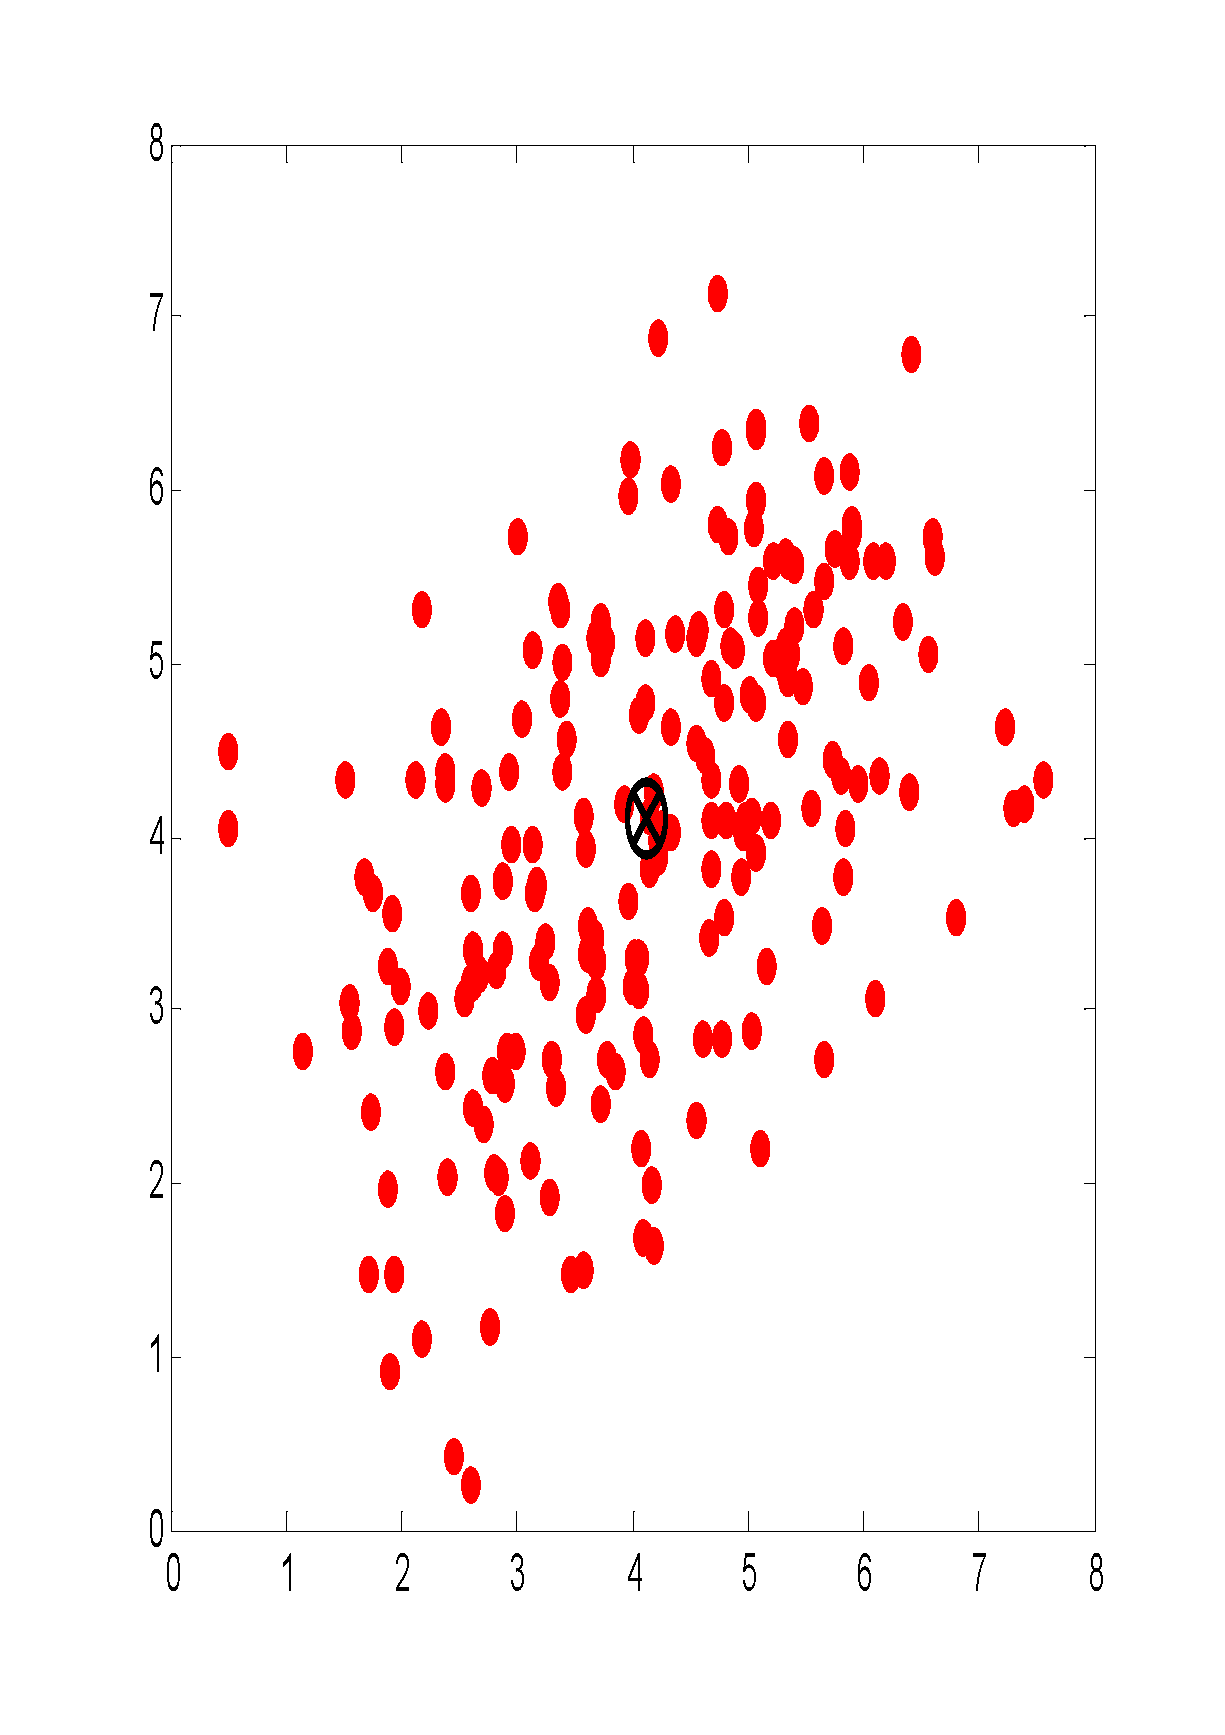
\includegraphics[bb=0mm 0mm 208mm 296mm, width=53.3mm, height=40.0mm]{image/image1.eps}\label{fig:fig2sub1}}
		\subfloat[][]{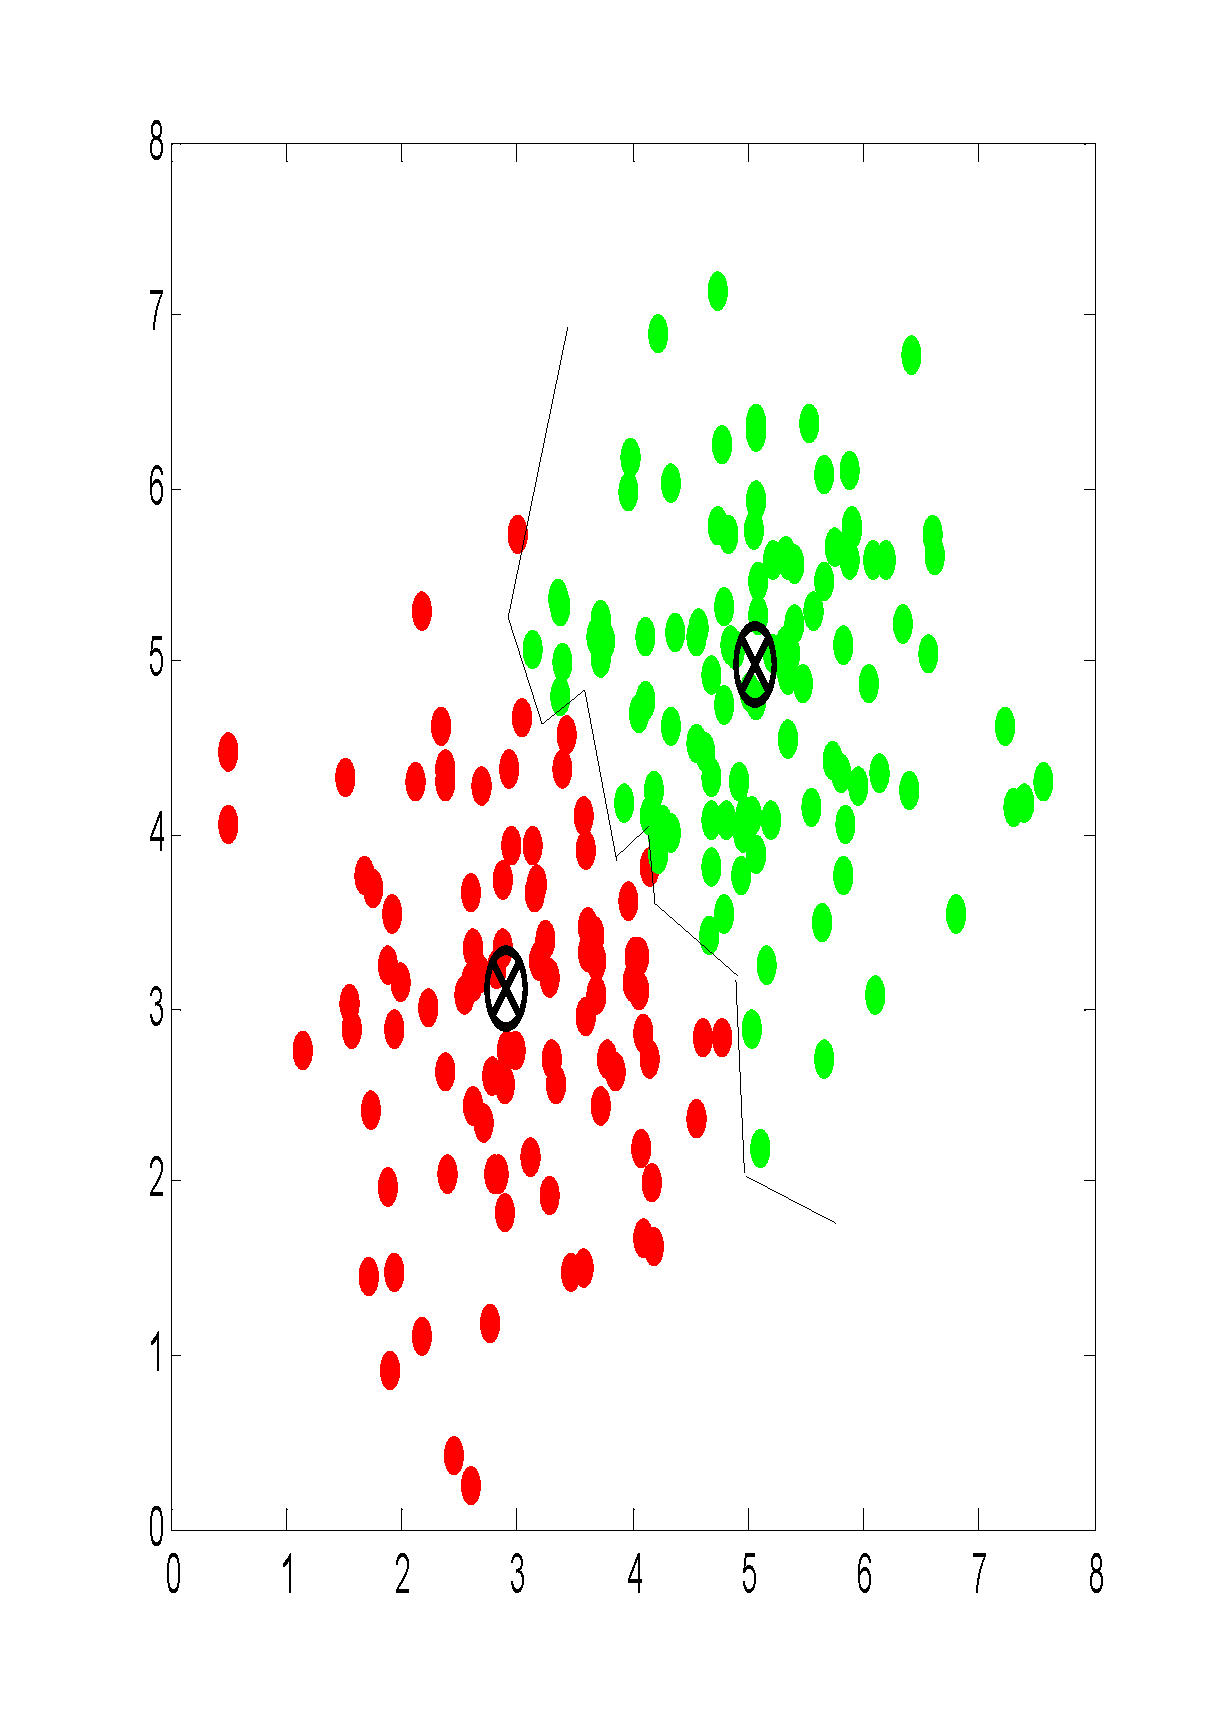
\includegraphics[bb=0mm 0mm 208mm 296mm, width=53.3mm, height=40.0mm]{image/image2.eps}\label{fig:fig2sub2}}
		\subfloat[][]{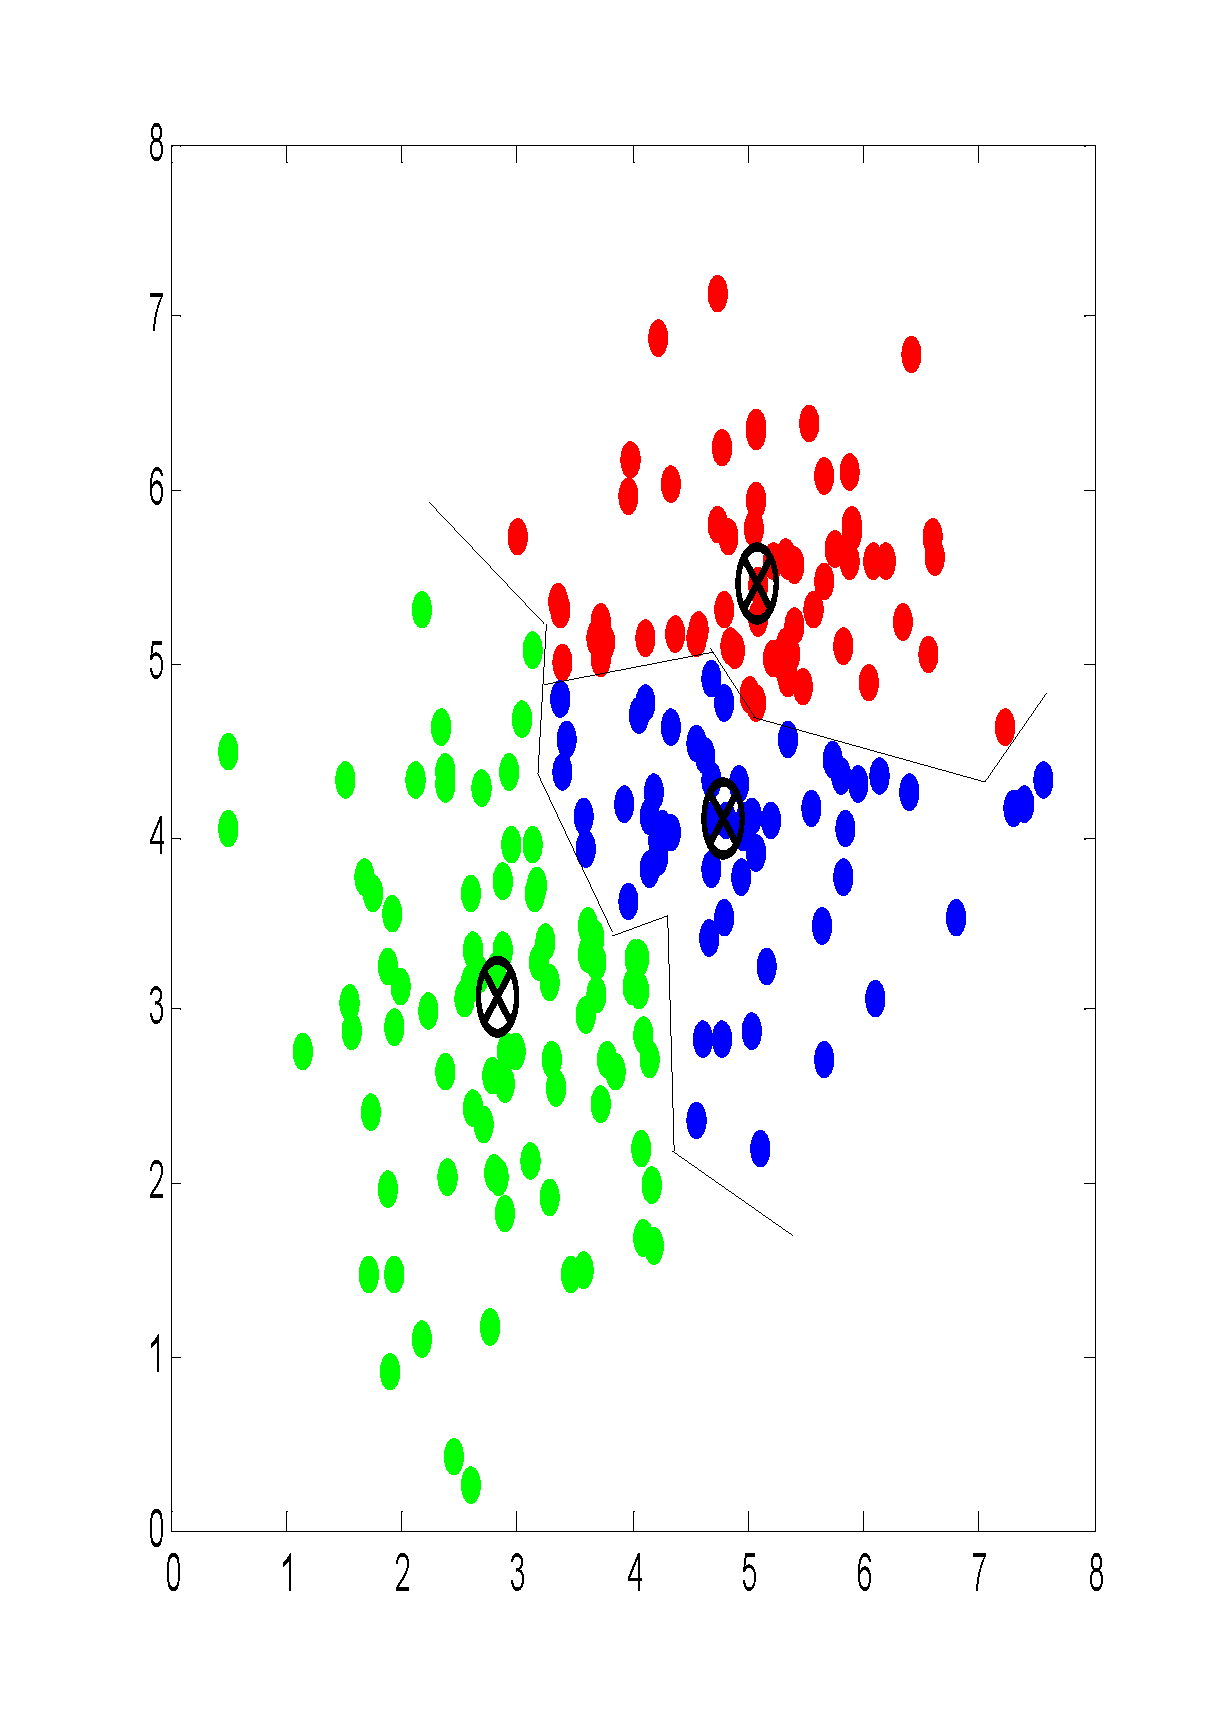
\includegraphics[bb=0mm 0mm 208mm 296mm, width=53.3mm, height=40.0mm]{image/image3.eps}\label{fig:fig2sub3}} \\
		\subfloat[][]{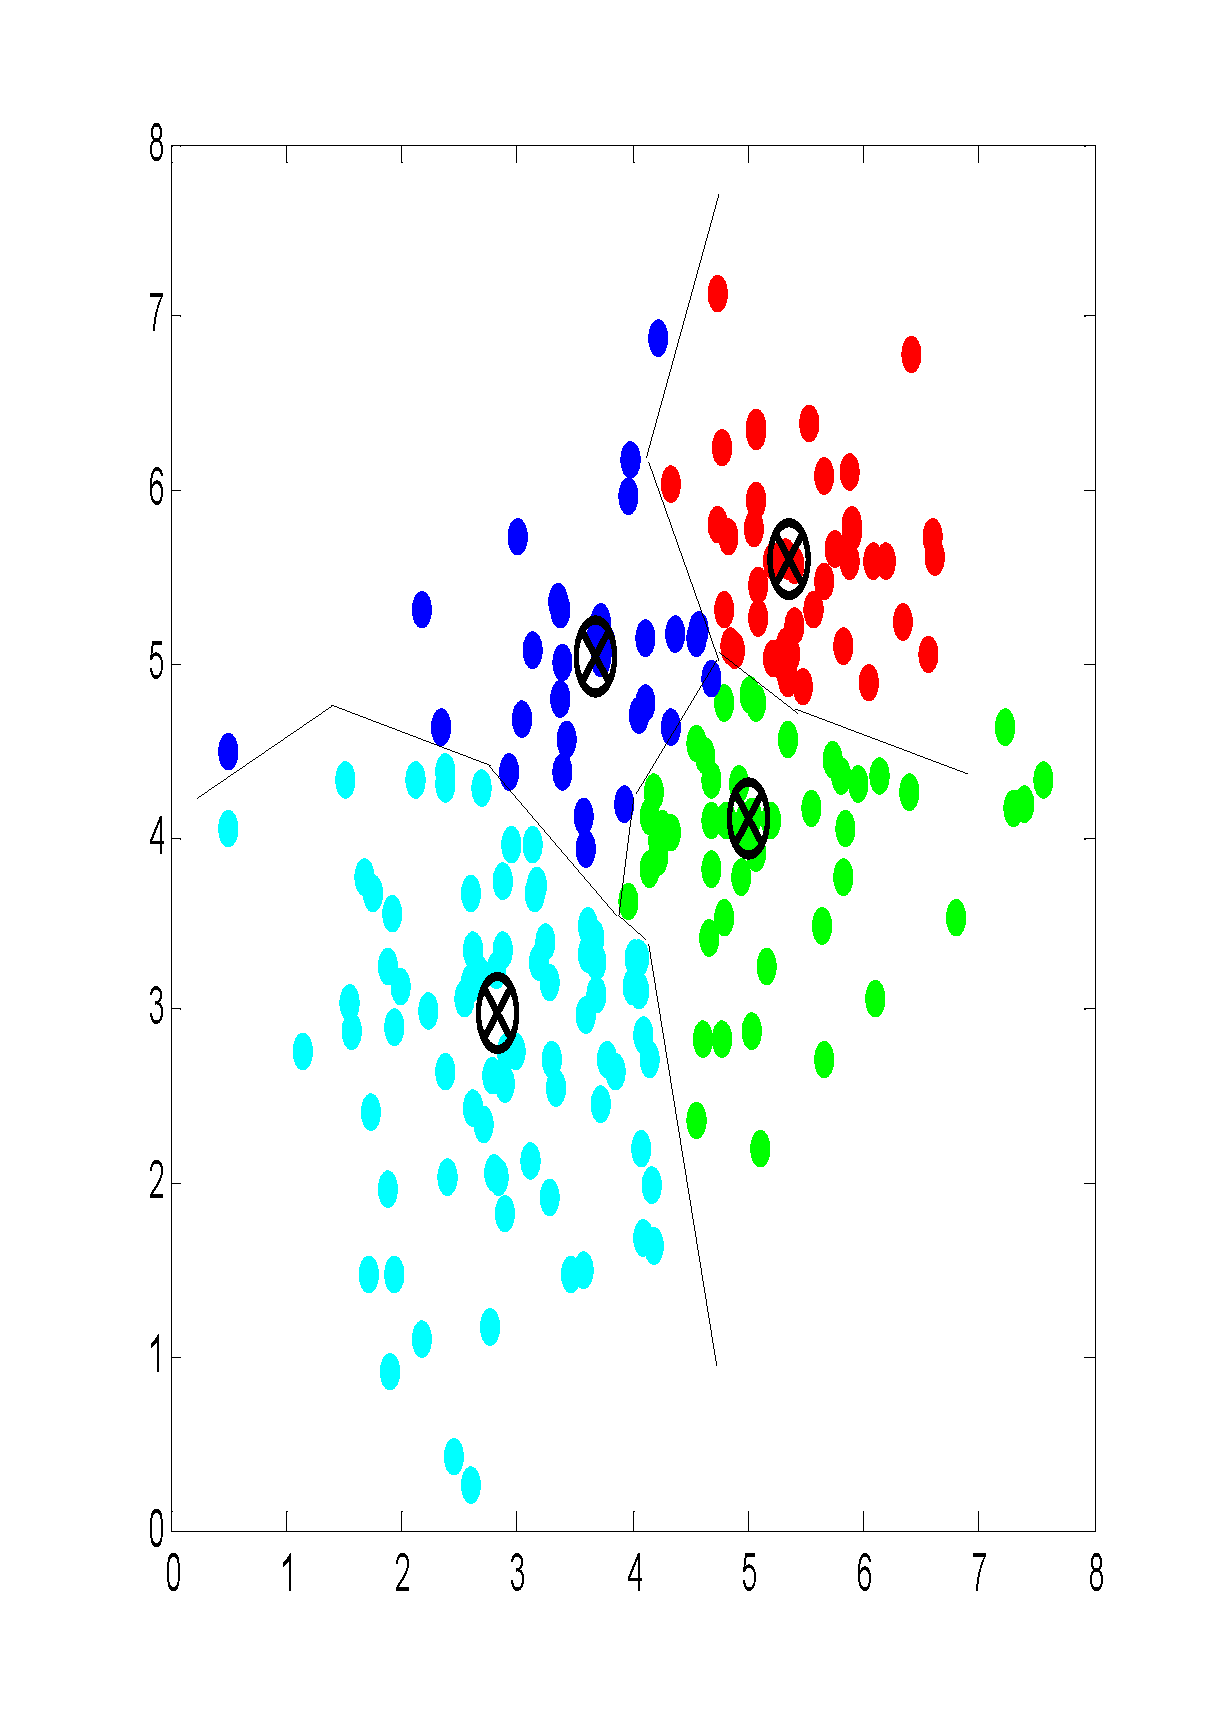
\includegraphics[bb=0mm 0mm 208mm 296mm, width=53.3mm, height=40.0mm]{image/image4.eps}\label{fig:fig2sub4}}
		\subfloat[][]{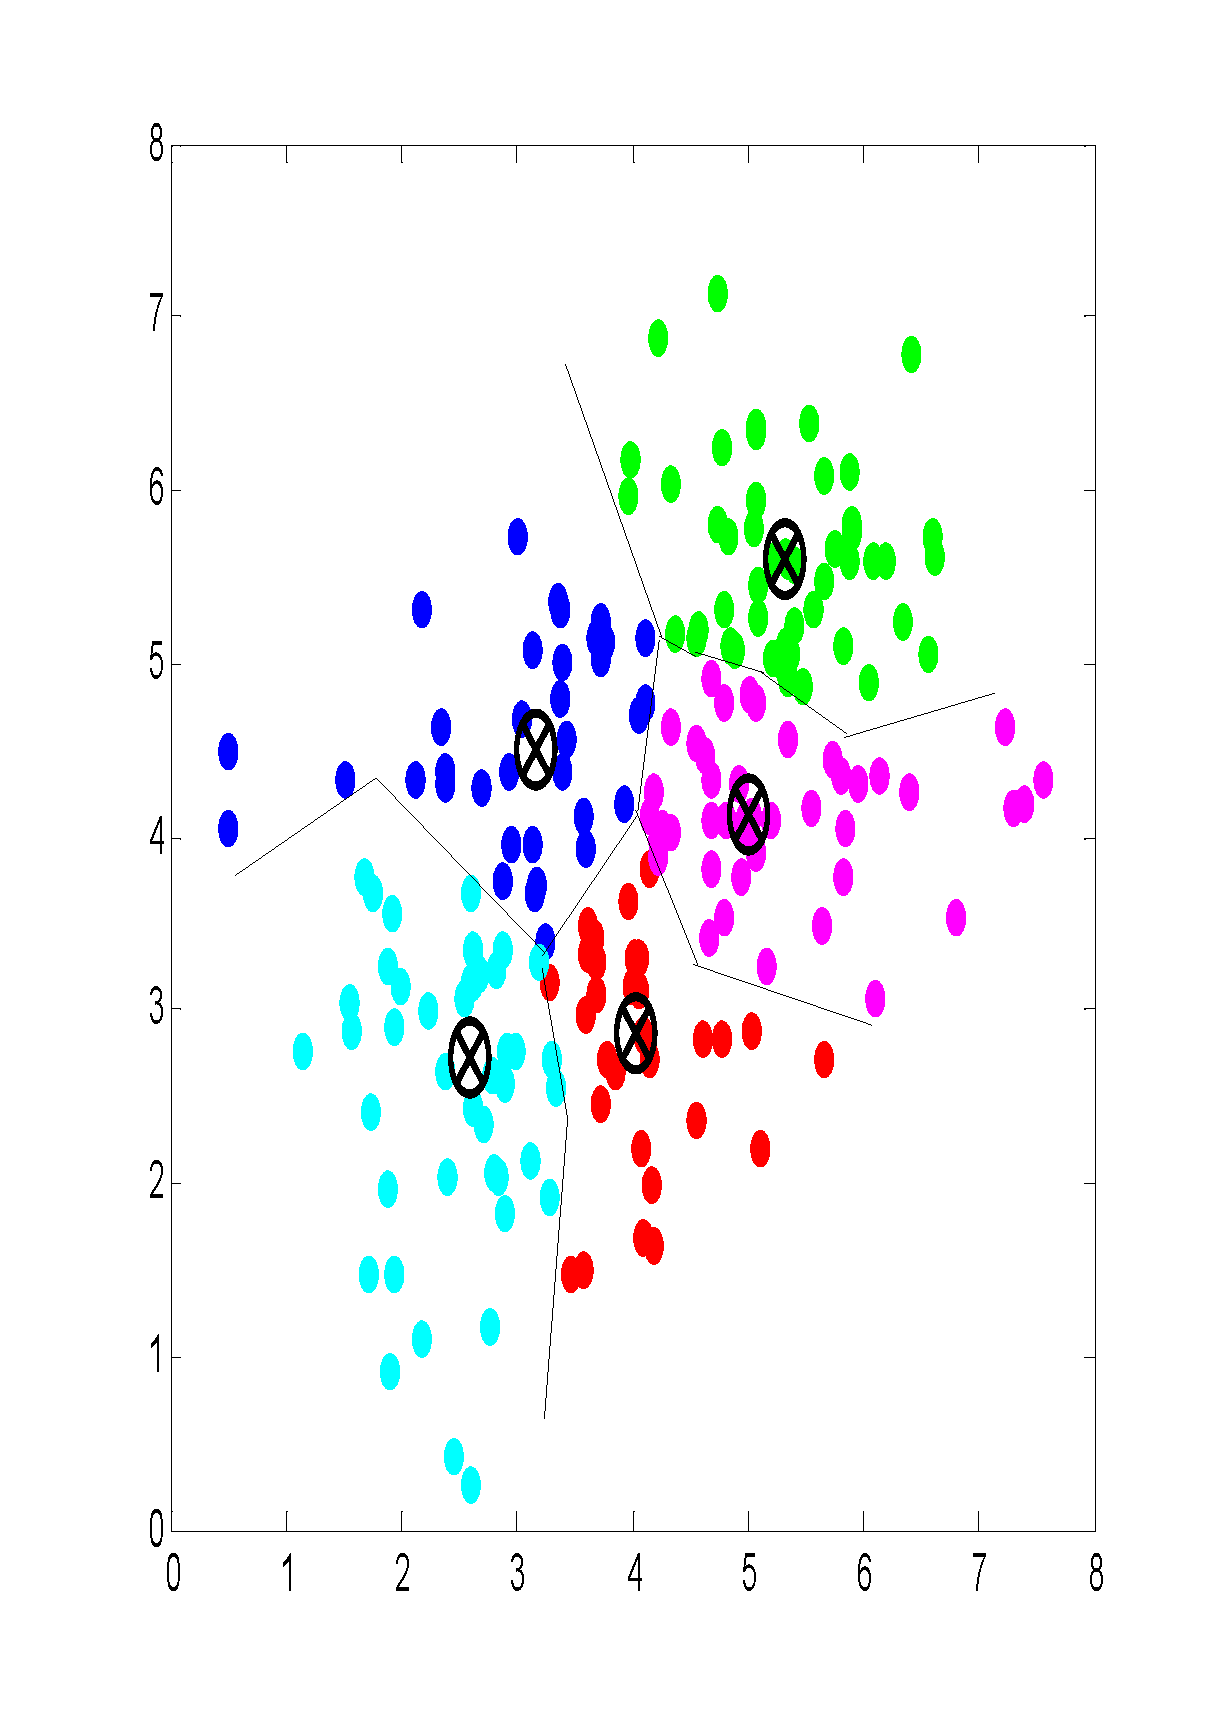
\includegraphics[bb=0mm 0mm 208mm 296mm, width=53.3mm, height=40.0mm]{image/image5.eps}\label{fig:fig2sub5}}
		\subfloat[][]{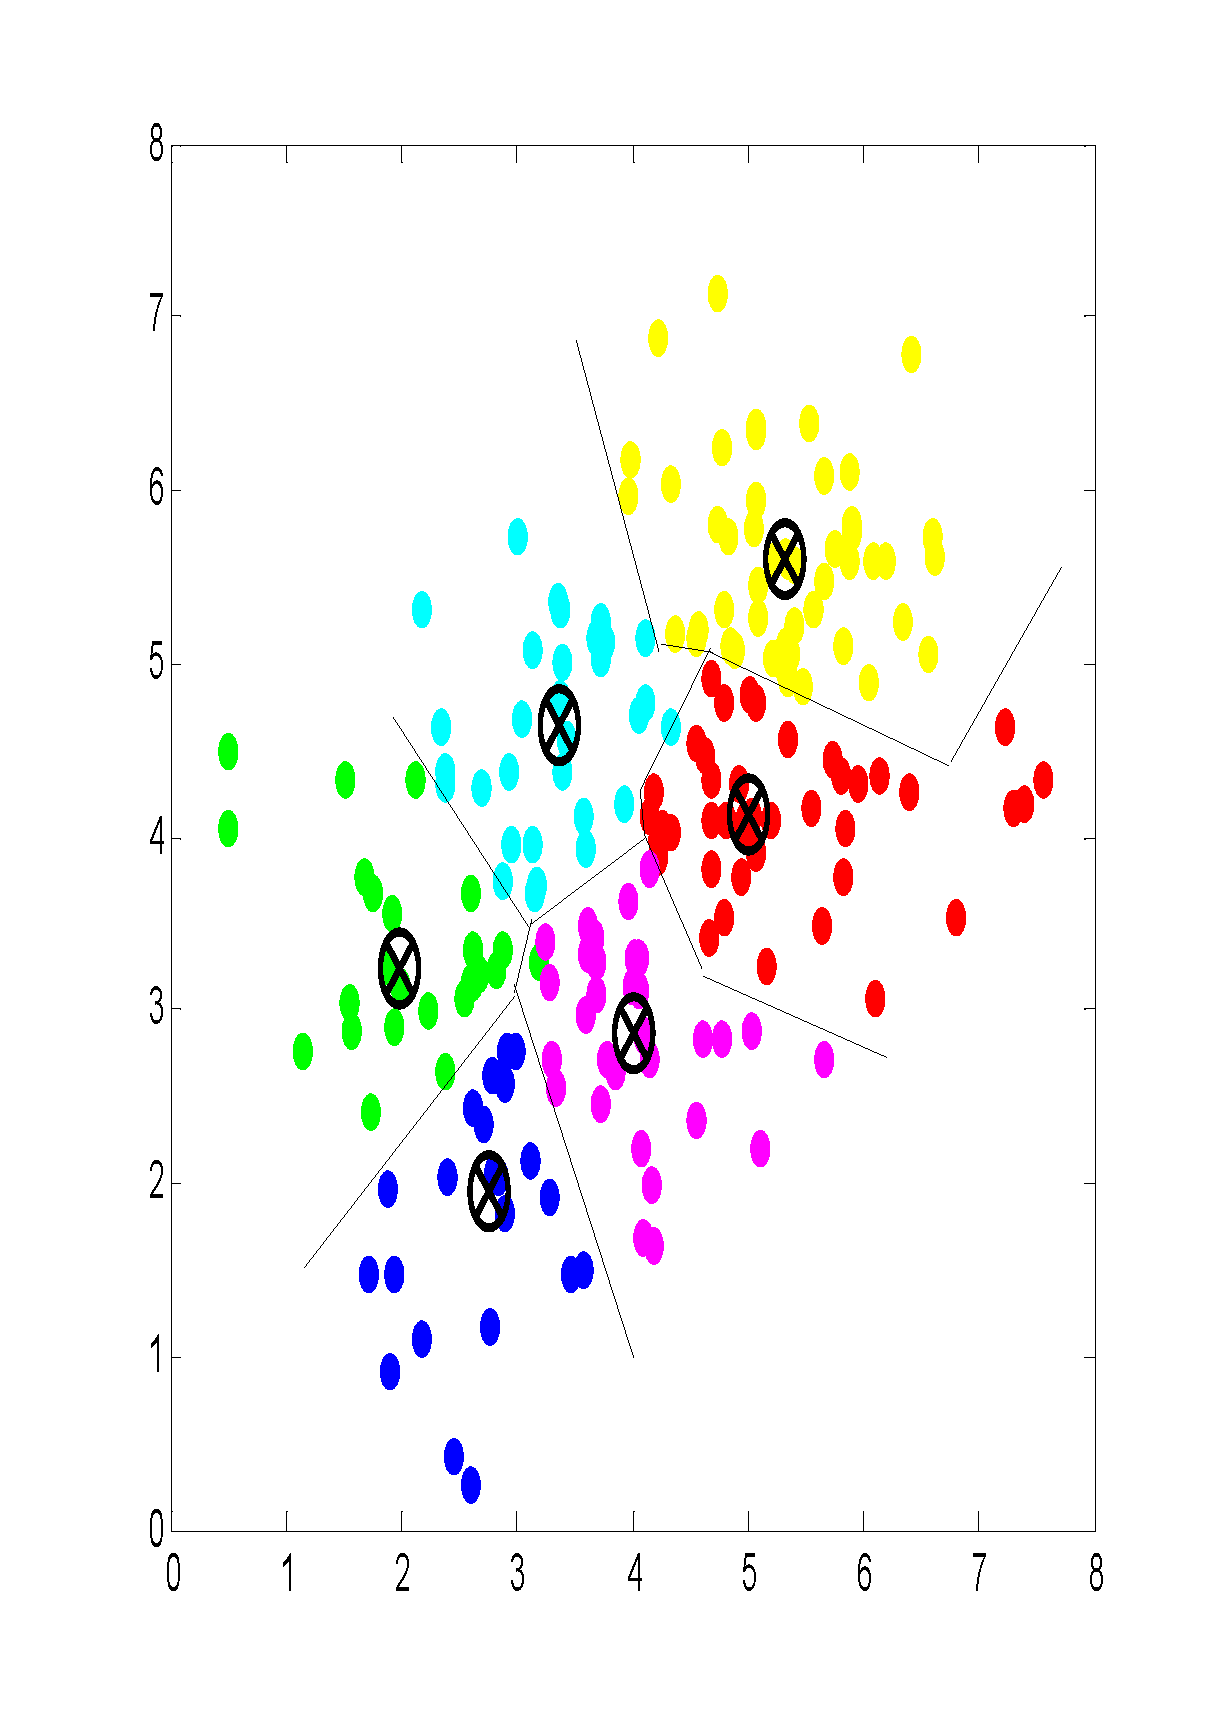
\includegraphics[bb=0mm 0mm 208mm 296mm, width=53.3mm, height=40.0mm]{image/image6.eps}\label{fig:fig2sub6}}
	\caption{CPU demand of 100 applications on a web server ($D_{w,i}$) on vertical axis vs. database server ($D_{d,i}$) on horizontal axis.}
	\label{fig:fig2}
\end{figure*}

\section{Dynamic Clustering of User Classes}
It seems natural to try to group the service instances with similar resource usage into a smaller number of classes and to control the modeling error. Since the resource demands associated with each service may change with time (i.e. due to changes in the system, workload dependant service demands, etc) we propose an adaptive clustering that regroups the service instances depending on the time-varying demands. The estimation filters track these changes, and the performance model predicts their effect on quality of service (e.g., on response time of different services).
A \textit{workload classifier} and a \textit{state estimator} group execution paths into runtime classes resulting into a new model with smaller set of classes. This model exploits the trade-off between \textit{complexity} (lessened by having a smaller set of modeled classes) and \textit{accuracy} (grows with the number of modeled classes). The role of \textit{state estimator} is to update and track estimates of the model parameters (e.g., service demands). 

An online tuned multi-class performance model will provide better control of application performance since it can estimate and predict the effect of decisions for each service offered by the application (as opposed to an average across all services).       

The original contributions presented in this section are:
\begin{enumerate}
\item  Estimation of hidden per class performance states for multi-class models
\item  Dynamic workload classification
\item  Evaluation of the effectiveness of approximation methods needed to make the classification and the multi-class estimator practical
\item  The interaction of the rate of system change, in determining the accuracy of classification and tracking 
\end{enumerate}

%\section{Dynamic Classification and Estimation}
%\label{sec:dynamic-classification-and-estimation}
%This section will present our classification and estimation methodology. 
% 

\subsection{Dynamic Clustering Algorithm}
\label{sec:dynamic-clustering-algorithm} 
In this section, we first discuss the modeling error due to clustering and then present an algorithm to determine the best choice of the number of clusters $C$ and the grouping of service instances into these clusters.

\subsubsection{Modeling Error} 
\label{sec:modeling-error} 
Suppose there are $C$ clusters (i.e. $c=1,\dots,C$), and $L$ service instances (i.e. $i=1,\dots,L$) and $c(i)$ denotes the cluster (or class) which contains service instance $i$. Let $R_{c(i)}$, the predicted mean response time of class $c(i)$ requests, 
be the basis for defining the error.\footnote{Other observed parameters which are model outputs such as throughputs $X_c$, per server response time $R_{c,k}$
server utilization ($U_{c,k}$ or $U_{k}$), or number of requests in a queue ($Q_{c,k}$ or $Q_{k}$ can also be used.}
 For the case of no clustering (i.e., each service instance is treated as a separate class), let ${R(L)}_i$ be the mean measured response time of requests for service instance $i$. Then a modeling error measure $E(C)$ for $C$ clusters is given by:

\begin{equation}
	E(C)=\sqrt{\frac{1}{L}\sum^L_{i=1}{{\left(\frac{{R(L)}_i-\ R_{c\left(i\right)}}{{R(L)}_i}\right)}^2}}
\end{equation} 

The hypothesis is that the error $E(C)$ tends to decrease when the number of clusters is increased. However, finding the clusters and the multi-class performance model associated with the clusters is complex as $E$ is a measure of how well the results from the filter and the model fit the measured data.

\subsubsection{Dynamic Clustering Algorithm} 
\label{sec:dynamic-clustering-algorithm-sub} 
Our classification algorithm is shown in  Algorithm \ref{estimation-algorithm1}. Input to this algorithm are the model, a measurement vector $z$ and an error threshold A. 
%The vector $z$ can include workload elements ${\lambda }_i$, the measured response time $R^m_i$ for service instance $i$ ($i = 1, 2, \dots , L$) and the total utilization of the servers $U_j$ ($j = 1, 2, \dots , J$).  
The algorithm outputs the best values of the number of clusters $C$ and the grouping of service instance's into these clusters (or classes) in terms of modeling error and modeling complexity, and the service time estimates at the various servers for each of the $C$ classes.  

\begin{algorithm}
	\small
	\SetAlgoVlined
	\SetKwInOut{Input}{input}
	\SetKwInOut{Output}{output}
	\SetKwInOut{Initialize}{initialize}
  \SetAlFnt{\tiny}

\Input{LQM, $z$, $A$}
\Output{The best choice of the number of clusters $C$, aggregated demand ($D_{j,c}$) and service instance members of clusters}
\BlankLine

Estimate $D_{j,i}$, the service demand of service instance $i$ at server $j$, from measurement data  ($\forall j\in\{1, \dots,J\}$, $\forall i\in\{1, \dots,L\}$) using the model with no clustering;
and set $C$ = 1.
\BlankLine
Cluster the service instances based on the $D_{j,i}$'s into $C$ clusters.  
\BlankLine
Estimate the parameters $D_{j,c}$, the service demand of class $c$ at server $j$; solve the LQM with $C$ classes and obtain results for $R_c$, the mean response time of class $c$ ($\forall j\in\{1, \dots,J\}$, $\forall c\in\{1, \dots,C\}$).  
\BlankLine
Calculate the modeling error $E(C)$
\BlankLine
If $E(C) > A$, then increase $C$ by $1$ and go to Step 2.
\BlankLine
Return $C$, the service instances in cluster $c$, and $D_{j,c}$ ($\forall j\in\{1,�,J\}$, $\forall c\in\{1,...,C\}$) 
\BlankLine

\caption{Estimation and Classification Algorithm.}
\label{estimation-algorithm1}
\end{algorithm}

In our investigation, the workload $W_i$ is time-varying. The estimation is executed at regular intervals. If the modeling error of the estimation for existing clustering configuration is less than $A$, only the regular estimation is performed using the Kalman filter. On the other hand, if modeling error is greater than $A$, our classification algorithm is invoked to obtain a new clustering of service instances such that the modeling error becomes less than $A$.             

The classification algorithm starts by estimating the service demands of all the service instances at the various servers from the measured response times using a model with no clustering (Step 1). 
% The service demand of service instance $i$ at server $j$ is denoted by $D_{j,i}$ ($\forall j\in \{1, \dots,J\}$, $\forall i\in \{1,\dots ,L\}$). 
The estimation is done by using the Extended Kalman filter to derive the hidden state parameters (the service demands in this case) from the measures that are available. 

%We also use multi-class model as the model component in the Extended Kalman filter structure. This model maps the state parameter vector $x$, composed of service demands $D_{j,i}$, and the workload parameters $W_i$ to output parameters $y$ such as mean response time of each service instance and utilization of each server, as given by the relationship $z=h(x)$. 
[do more explanation ....]


In Step 2, the K-means clustering algorithm \cite{kaufman_finding_1990,likas_global_2003} is used to perform unsupervised grouping of service demands. K-means has a low complexity and is adaptable to a continuous nature of workload classification problem. Moreover, it is able to detect clusters in an efficient way which does not require computing the distance of all points in space to each other. K-means takes as input the number of distinct clusters to generate ($C$) and will determine the size of the clusters based on the structure of the data. 

The modeling error $E(C)$ is calculated at Step 4 using analytic results for $R_c$ obtained in Step 3. If $E(C)\le A$, the algorithm terminates and returns $C$, the service instance assigned to each of the $C$ clusters, and the estimated service parameters for the different classes (see Step 6). 

Step 5 corresponds to the situation where the modeling error $E(C)$ is larger than the acceptable error $A$. This is usually a result of gradual changes in service demands over time. Here the algorithm re-calculates the clusters; this may lead to a larger number of clusters (more estimation precision) or reshaping with the same number of clusters. Both approaches can improve the accuracy of estimation and decrease the error. Steps 3 and 4 are then repeated to compute $E(C)$ for the clusters obtained from re-calculation. Note that a larger number of clusters would increase the computational cost of estimation, but it will decrease $E(C)$. 

\begin{figure}
	\centering
	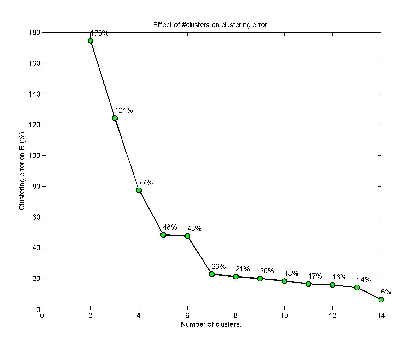
\includegraphics[width=0.45\textwidth]{image/modeling-error-vs-num-cluster.eps}
	\caption{Modeling error decreases with the number of clusters.}
	\label{fig:fig6}
\end{figure}

\subsubsection{Number of Clusters and Modelling Error} 
To asses the effect of number of clusters on the modelling we demonstrate two main analyses.  

% \par \textbf{Number of Clusters versus Error}
First we ran the algorithm statically with different number of clusters and measured the modeling error. In our evaluation, we used an expanded definition of the error metric given by its average value over the duration of the experiment (from $t_1$ to $t_2$): 
\[E=\frac{\sum^M_{step=1}{{E(C)}_{step}}}{M}\] 
where $step$ is a variable which ranges over the estimation steps. $E(C)$ is the modeling error defined in subsection \ref{sec:modeling-error} and $M$ is the number of estimation steps. 

As we expected, the error decreased while we increased the number of clusters (see Figure 6). The experiment also shows that modeling the system with one or even two classes introduces a large modeling error and that modeling with an intermediate number of classes (8,  for example) might give us an acceptable modeling error. 

%\begin{figure}
%	\centering
%	\includegraphics[width=0.45\textwidth]{image/cluster_kum_by_error.eps} 
%	\caption{The minimal number of needed clusters to reach certain modeling error.  We can reach 40\% and 17\% error, consecutively using 9 and 12 clusters on average. In order to reach 5\% error we have to perform full clustering.}
%	\label{fig:fig7}
%\end{figure}
%
%% \par \textbf{Number of Clusters versus Error} 
%In the second analysis, we applied our estimation and clustering algorithm to find the minimal number of needed clusters to reach certain modeling error. The algorithm is applied at each sampling period and, as a result, the clusters change dynamically.  As Figure 7 shows, we can reach 17\% error using between 7 and 12 clusters for the duration of the experiment. For a modeling error less than 40\% we need 9 clusters on average. In order to reach 5\%, there are sampling periods in which we need maximum number of classes.

\subsubsection{Shape of Clusters versus Error} 
The third analysis observed the correlation between the within cluster sum-of-squares (WCSS) for demands and the modeling error achieved using the Estimation and Classification Algorithm. We chose 140 different groupings (for each number of clusters we generated 10 random combinations). This let us navigate all possible WCSS's that could result from different groupings. Figure 8 shows that, on average we experienced a larger modeling error for the clusters with higher WCSS error. In other words, the modeling error is minimized, whenever the WCSS is minimized. As a result, our assumption is validated since K-means is exactly the algorithm to minimize the WCSS. 

\begin{figure}
	\centering
	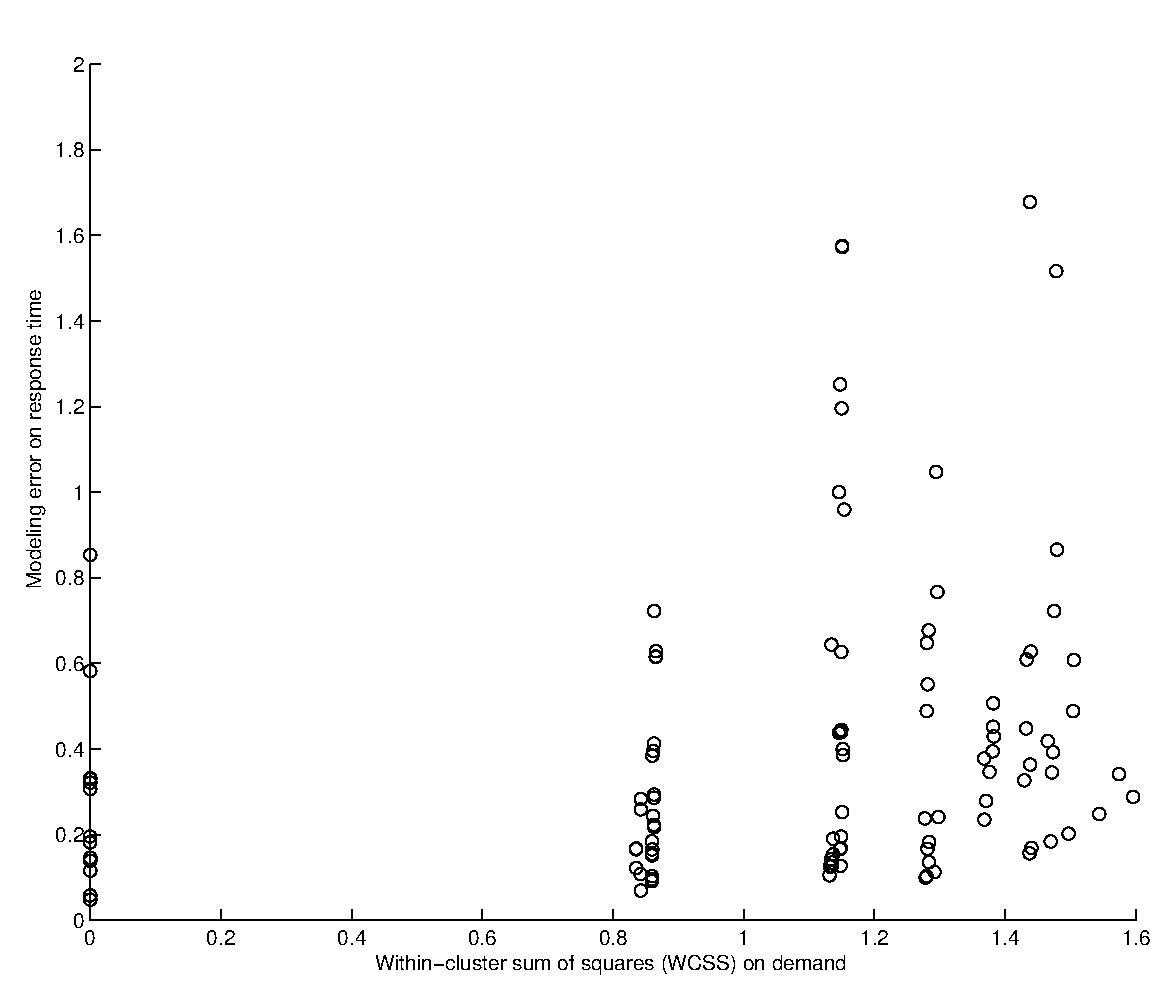
\includegraphics[width=0.45\textwidth]{image/clustering_error_corelation.eps} 
	\caption{Correlation between WCSS for demands and the error achieved on response times estimation.}
	\label{fig:fig8}
\end{figure}

\subsection{Example 1: TPCW benchmark and FIFA workload}  
TPC-W is a web application composed of 14 URLs, each having different service demands on web and database servers, and a workload defined in terms of percentage of total number of users.  The benchmark has three workload mixes, buying, ordering, and browsing. Based on the workload mix the distribution of workload amongst URLs varies. This workload is generated using emulated browsers (EBs) whose behavior and navigation is controlled by a Markov chain with certain probabilities to match the desired distribution of load between URLs. As a result, there is a Markov chain per user mix. 

\begin{figure}[tp]
	\centering
		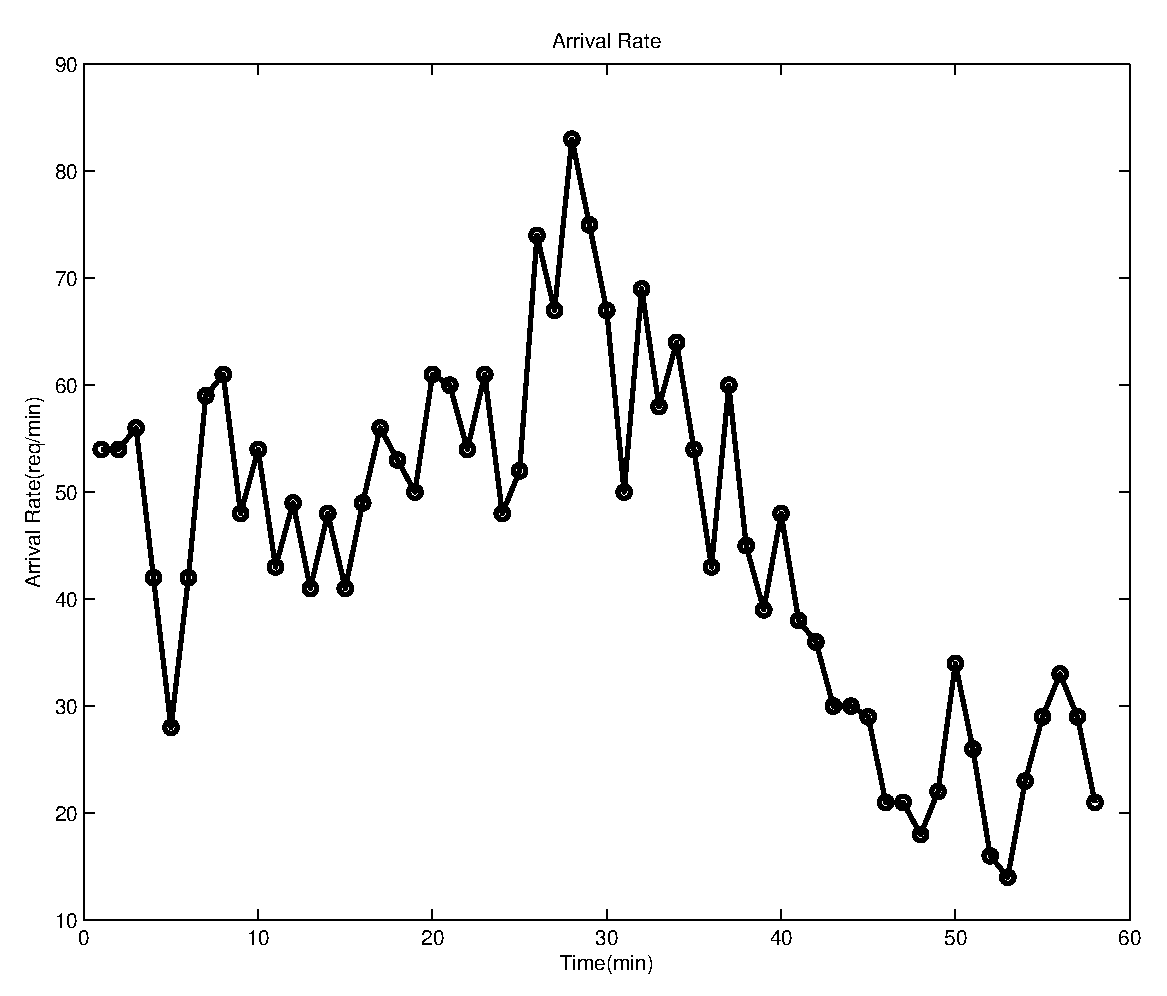
\includegraphics[width=0.45\textwidth]{image/workload-arr-rate.eps}
	\caption{FIFA98 workload, day 21, over an hour.}
	\label{fig:fig5}
\end{figure}

%We deployed the Java implementation of TPC-W \cite{volker_turau_tpc-w_????} with some modification, on a cluster of four Tomcat web servers and one single MySQL database server, with Linux as the operating system.  
In order to be realistic, we used FIFA98's \cite{arlitt_workload_2000} workload instead of TPC-W's original workload. 
% The TPC-W's original workload is just to test scalability but 
FIFA98 reflects variations that servers might experience at runtime. We picked a portion of the day $21^{\text{st}}$'s workload (see Figure 5), extracted the web pages, lowered the number of requests with the factor of 2 (to factor in our smaller scale deployment topology), and finally used the Little's law \cite{little_proof_1961}  (i.e. $N=X(R+Z)$) to convert the obtained throughput ($X$) to the number of users ($N$) and think time ($Z$) used by emulated browsers of TPC-W. In this conversion we assumed that FIFA98 website had maintained the same response time over the sampling period. We then used the obtained number of users to the TPC-W benchmark using equal mix of buying, browsing, and ordering scenarios. 

For obtaining data, we monitored one of the web servers and the database and logged response times, throughputs, utilizations plus the workload parameters. Each sample represented a minute of work and the total length of experiment was 1 hour resulting into 60 samples.

We noticed that under this workload, the demands do not change frequently, and suspected that this is mainly because 1) the workload is unable to fully saturate the system or 2) the fact that combination of workload mixes are the same.

\begin{figure}
	\centering
	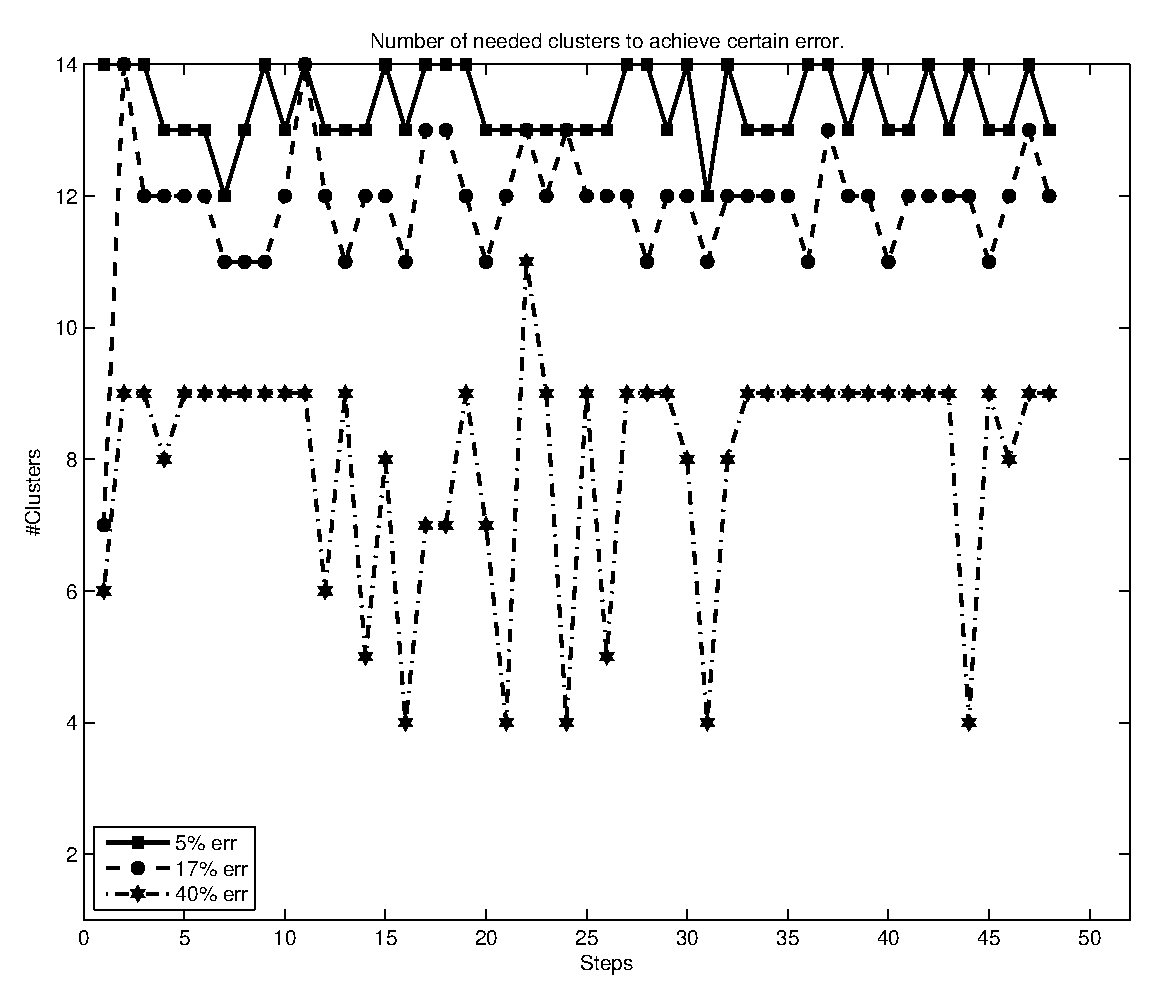
\includegraphics[width=0.45\textwidth]{image/cluster_num_by_error.eps} 
	\caption{The minimal number of needed clusters to reach certain modeling error.  We can reach 40\% and 17\% error, consecutively using 9 and 12 clusters on average. In order to reach 5\% error we have to perform full clustering.}
	\label{fig:fig7}
\end{figure}

We applied our estimation and clustering algorithm to find the minimal number of needed clusters to reach certain modeling error. The algorithm is applied at each sampling period and, as a result, the clusters change dynamically.  As Figure 7 shows, we can reach 17\% error using between 7 and 12 clusters for the duration of the experiment. For a modeling error less than 40\% we need 9 clusters on average. In order to reach 5\%, there are sampling periods in which we need maximum number of classes.


\subsection{Example 2: Simulated Workload with Highly Variable Demands}  
\label{sec:estimation-highly-variable-demands} 
In TPC-W experiment, the service demands did not vary in short run. As a result, it was unlikely that a service instance moved from one cluster to another very often. However, in a long run (e.g.~a month in real system measures) service instances might change place due to variation in the database records they access or in change of service instance parameters. In short run, service instance parameters variations may change the demands as well.

We performed a simulated experiment for such a case to investigate the effectiveness of the algorithm under non-uniform variations in demands. The simulator software used was CSim discrete event-based simulator. 

To keep the presentation simple but also to highlight the merits of the proposed method, in the simulation we varied $Z_c$ and the CPU demands, and kept $N_c$ and the request frequencies constant. 

\begin{figure}[htbp]
	\centering
   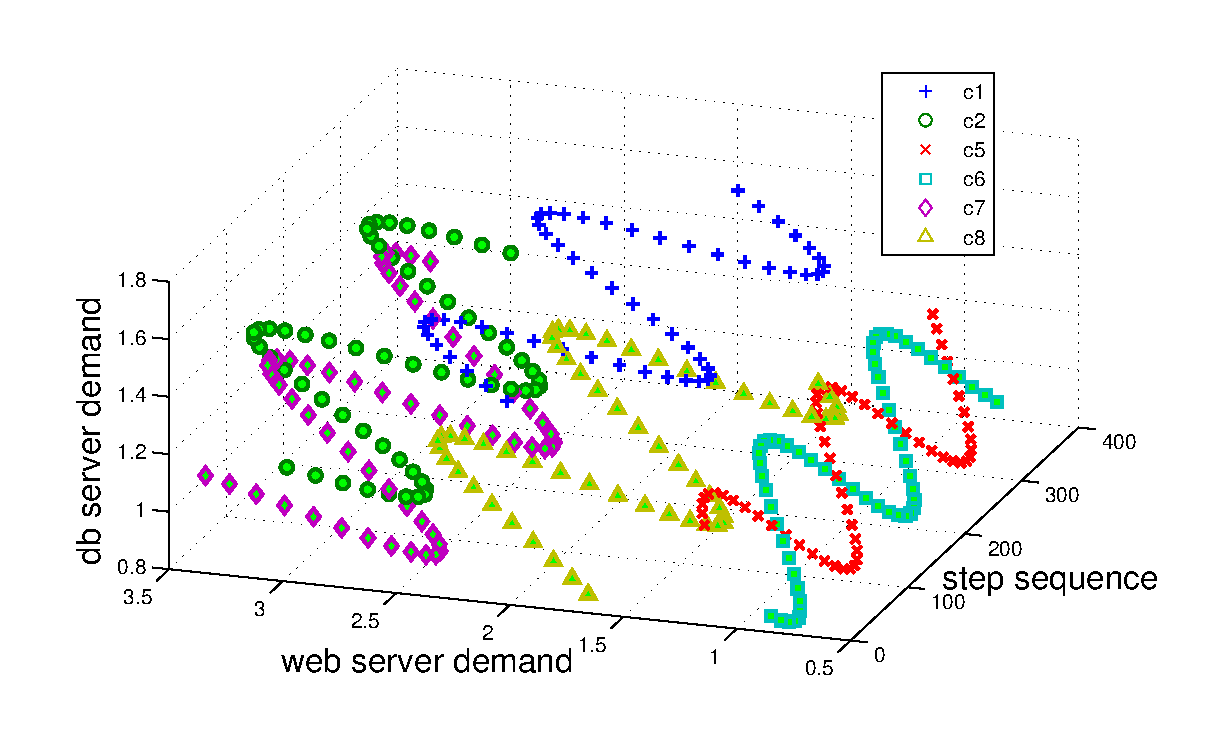
\includegraphics[width=0.45\textwidth]{image/variation-of-service-demands6.eps}
	\caption{Combined Web-DB service demands for a specific set of classes [c1,c2,c5,c6,c7,c8].}
	\label{fig:fig9}
\end{figure}


This experiment shows the efficiency of clustering and estimation for a web based application when the estimated parameters change at different rates and phases (small change in service demands). This web based application is an e-commerce site with 8 service instances (browse, buy, checkout, admin, login, logout, add, and remove). The service instances have the same number of users ($N_c$), mean user think time ($Z_c$), and time variant service demands $D_{w,c}$ and $D_{d,c}$. Service demands follow the sine curve with the same period but different phases (see Figure 9). Because of demand variations, service instances migrate from one cluster to another and clusters evolve over time. In real applications, the service demands are not going to change that dramatically, we consider those variations as a stress load on the algorithm. Because of the variation of the service demands, we expect that the different classes will be re-clustered periodically.                                                                     

\begin{figure}[tb]
	\centering
	\subfloat[][]{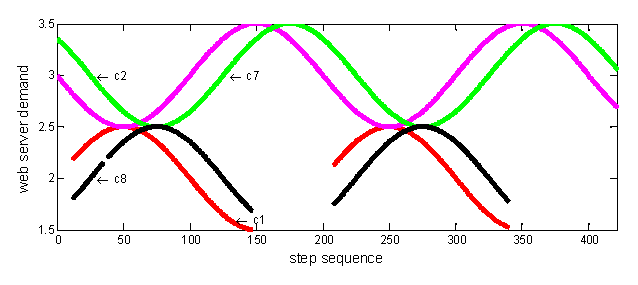
\includegraphics[width=0.45\textwidth]{image/variation-of-service-demands.eps}\label{fig:demands-sub1}} \\
	\subfloat[][]{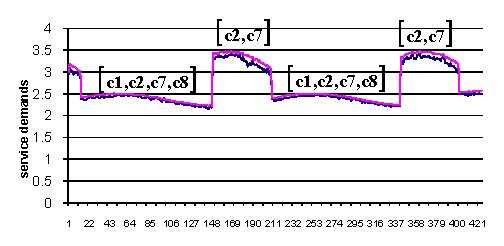
\includegraphics[width=0.45\textwidth]{image/real-and-tracked-service-demands2.eps}\label{fig:demands-sub2}} \\
	\subfloat[][]{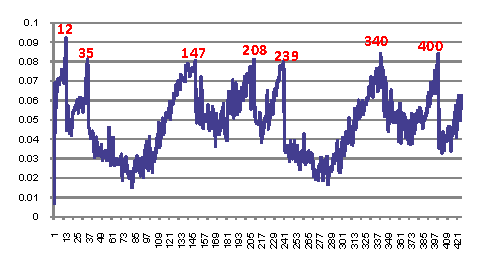
\includegraphics[width=0.45\textwidth]{image/the-modeling-error.eps}\label{fig:demands-sub3}} \\
	\caption{Variation of service demands in (a),
% Real and Tracked Service Demands for one cluster in (b)
%and the modeling error in (c).
real and and tracked service demands for 2 clusters [c2,c7] and [c2,c7,c1,c8] in (b), 
and modeling error with dynamic clustering applied in (c).
}
	\label{fig:fig10}
\end{figure}


\begin{table}
	\centering
\begin{tabular}{|p{0.3in}|p{0.4in}|p{0.9in}|p{0.8in}|} \hline 
Step & Action\newline Nature & Grouping\newline (Pre-event) & Grouping (Post-event) \\ \hline 
12 & Ag, Mv & [c1,c5,c6,c8] [c2,c7] [c3] [c4] & [c1,c2,c7,c8] [c3,c4]  [c5,c6] \\ \hline 
35 & Br & [c1,c2,c7,c8] [c3,c4] [c5,c6] & [c1,c2,c7,c8] [c3] [c4] [c5,c6] \\ \hline 
147 & Mv & [c1,c2,c7,c8] [c3] [c4] [c5,c6] & [c1,c5,c6,c8] [c2,c7][c3][c4] \\ \hline 
208 & Ag, Mv & [c1,c5,c6,c8] [c2,c7] [c3] [c4] & [c1,c2,c7,c8] [c3,c4] [c5,c6] \\ \hline 
239 & Br & [c1,c2,c7,c8] [c3,c4] [c5,c6] & [c1,c2,c7,c8] [c3] [c4] [c5,c6] \\ \hline 
340 & Mv & [c1,c2,c7,c8] [c3] [c4] [c5,c6] & [c1,c5,c6,c8] [c2,c7][c3][c4] \\ \hline 
400 & Br, Mv & [c1,c5,c6,c8] [c2,c7] [c3] [c4] & [c1,c2,c7] [c5,c6,c8] [c3,c4] \\ \hline 
\end{tabular}
	\caption{Changes in clustering structure during simulation.}
	\label{tab:h}
\end{table}

Table 1 shows the clusters suggested by K-means algorithm. The acceptable modeling error A is set to 8\% over 421 simulation steps. The column `Action Nature' indicates the kind of change that has occurred when the past and current clustering are compared; Ag, Br, Re, and Mv stand for aggregation, breaking, re-structuring, and movement respectively. Notice that in each re-clustering, the clusters are re-computed from scratch; meaning that the algorithm is oblivious to `Action Nature'. 

Figure 10(a) shows the variation of service demands in a changing cluster ([c2,c7]+[c1,c8]). Real and tracked service demands for the cluster are shown in Figure 10(b) while the modeling error is depicted in Figure 10(c). 

According to Figure 10(a) and demand formulas, at step 50, $(D_{w,1},D_{d,1})$ and $(D_{w,2},D_{d,2})$ get close. This suggests that c1 and c2 should be in the same cluster near that step. At step 150, the service demands of c1 and c2 are quite different, indicating that these two classes are more likely in different clusters. These observations are consistent with our results where the clustering at step 50 is [c1,c2,c7,c8][c3][c4][c5,c6] and [c1,c5,c6,c8][c2,c7] [c3][c4] at step 150. Notice that c1 and c8 are shown in Figure 10(a) only when they are part of the cluster [c2,c7,...]. This explains the step-function-like behavior of the estimated demand for the changing cluster in Figure 10(b).

\begin{figure}[htbp]
	\centering
	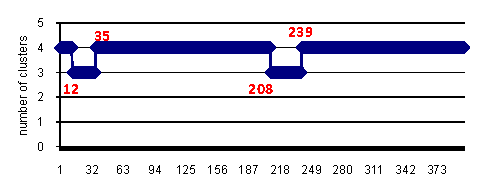
\includegraphics[width=0.45\textwidth]{image/number-clusters-versus-simulation-steps.eps}
	\caption{Number of clusters versus simulation steps.}
	\label{fig:fig11}
\end{figure}

Based on Figure 10(c) during the simulation, the modeling error exceeds the threshold $A$, 7 times. This means the classification algorithm described in subsection \ref{sec:dynamic-clustering-algorithm} is activated 7 times among the 421 steps. One could see that not every re-clustering necessarily results into a different~number of clusters. For example, at step 147, the clustering changes from [c1,c2,c7,c8][c3][c4][c5,c6] to [c1,c5,c6,c8][c3][c4][c2,c7]. The number of clusters remains the same, but c1 and c8 have been moved to a different cluster. Figure 11 shows that the total number of clusters changes only 4 times over the 400 steps.

We can conclude that our estimation and classification algorithm works quite well, since it is able to keep the error below $A=0.08$ with the smallest number of clusters and acceptable frequency of re-clustering. 

The algorithm also satisfies our claim in Section \ref{sec:introduction}: being able to exploit the complexity-accuracy trade-off and keeping both the error and the estimation cost low. In terms of cost, our algorithm yielded half the required clusters (see Figure 11) compared to full service instances estimation, which from the theory reduces the estimation cost by a factor $2^3$ ($\frac{1}{2^3}$ of the original cost). This is due to the fact that, the cost of Kalman estimation in each step is dominated by Kalman gain calculation, which is $O(l^3)$ while $l$ is the number of measured variables. The reason is that the dominating term during gain calculation is a inversion of a matrix of size $l\times l$:

\begin{equation}
	K_k=P^-_k H^T_k{(H_k P^-_k H^T_k+R_k)}^{-1}
\end{equation} 

In this equation, $R_k$ is measurement noise covariance matrix with size $l\times l$.

In terms of accuracy, it was able to keep the error near zero compared to fully aggregated service instances case. See Figure 12 for the error comparison between our algorithm, one cluster case, and full service instances estimation. 
\begin{figure}[htbp]
	\centering
	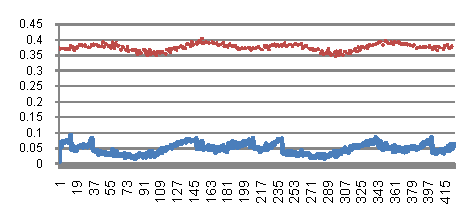
\includegraphics[width=0.45\textwidth]{image/comparison-modeling-error-one-cluster-dynamic.eps}
	\caption{Comparison of the modeling error for one cluster case (dotted line), dynamic clustering case (solid line), and full service instances estimation (solid horizontal line at $y=0$).}
	\label{fig:fig12}
\end{figure}

\section{Related Work} 
\label{sec:related-work}
Some of the early works in CPU demand estimation are done in \cite{rolia_parameter_1995} and \cite{rolia_correlating_1998}. They used regression analysis to predict demands of certain program in a distributed system. The reference \cite{courtois_using_2000} uses regression splines instead of linear and polynomial regression functions to better capture the irregularities of demand functions. References \cite{pacifici_cpu_2008,zhang_regression-based_2007} employ the multivariate linear regression technique for a one-tier network.  However, \cite{zhang_regression-based_2007} focuses more on modeling the inter-request dependencies of session-based systems and \cite{pacifici_cpu_2008} focuses on mechanisms to deal with issues such as insignificant flows, collinear flows, space and temporal variations, and background noise. In \cite{zhang_workload_2002} and \cite{liu_parameter_2006}, multi-class queuing models were used to infer the per-class service times at different servers of a two-tier web cluster using throughput, utilization, and per-class response time measurements. They try to minimize the sum of predicted response time mean square errors using a non-linear optimization solvers and quadratic minimization programs. References \cite{gmach_workload_2007,gmach_capacity_2007} claim to perform demand prediction of enterprise workloads by discovering patterns, but the referred demand is per-application not per-request; thus they do not tackle the same problem as ours. Finally reference \cite{kraft_estimating_2009} contributed by using Maximum Likelihood Estimation together with queuing model to estimate resource consumption in an ERP system.  

Our tracking filter based approach is closer to what we previously presented in \cite{woodside_use_2005,xu_performance_2005,zheng_tracking_2005}: it uses LQM which is adaptable to open and closed workload types, and is designed to be used in online estimation and control. However, theoretically our approach is applicable to regression based techniques as well. One can apply regression to track changes in service demands by continually reapplying the technique on new measurement samples and feed the result into our clustering algorithm. In this case regression can be tuned by adjusting the number of past samples used.

The major contribution of this paper is the dynamic estimation of multi-class model parameters and the dynamic clustering of user requests. To the best of our knowledge, the combination of dynamic clustering and cluster parameter estimation has never been investigated before. Only reference \cite{sharma_automatic_2008} is close to our work in terms of final goal. They try to categorize requests based on their resource usage characteristics without performing server instrumentation. Thus they ignore the prior knowledge of which service instance a request is accessing and only uses aggregate metrics such as total CPU usage over time. Moreover, their utilized approach is also different, as they use a machine learning technique called independent component analysis (ICA). Of course, their technique will erase the need for server instrumentation but might affect the accuracy due to not using the extra available information.


++++++

 
% \textit{Enhanced convergence}. The Iterated EKF (IEKF) [13] gives improved estimates for nonlinear $h(x)$ by linearizing $h(x)$ around the predicted state estimate $\hat{x}^-_k$ and iterating the update. Other variants which are (by experience) better for nonlinear $f(x)$ are the Unscented Kalman Filter [14] and the Divided Difference Filter [23].

% Thus in process of identification, two activities is performed simultaniously (i) building the model of relationship between theory and system input/outpus and (ii) estimating the ongoing state of the system in terms of the theory as new data becomes available. 

%\subsection{Future Work} 
%\label{sec:future-work} 
%In this paper, we used the maximum acceptable error value (8\%) obtained from experience to control the balance between the introduced error and complexity of the model (noting that our goal was to minimize both). As future work, one can model the relationship between computation complexity and error explicitly and try to find an optimal number of clusters which minimizes both.
%
%Another future challenge is the integration of multiclass model with the decision component of the adaptive loop. It is foreseeable that the decisions on provisioning to be made p
%
%

% The extended Kalman filter is a variant of the Kalman filter \cite{welch_introduction_1995} for a non-linear measurement equation.
% ++++++++++

%+++++++
%Predictive Model: A model of the system is developed to represent the relation between performance metrics   and the reservation actions ?_k. Essentially, we obtain the model of the form:
%x_(k+1)=f(x_k,?_k,w_k )
%y_k=g(x_k) 
%	(4)
%where w_kdenotes the workload and is considered a random term, ?_k is control variable, and x_kincludes several state variables of interest disscussed later. 
%In order to relate the amount of resources (?_k) to well-known performance metrics (y_k),  queuing theory and performance models [35, 24, 32] were used. In simplest case, PaaS is modeled as a simple  -server cluster handling transactional workload where service demands do not depend on the queue lengths. In this case the transient response time (the most common performance metric), can be modeled as a set of simple linear equations:
%r_(k+1)=(1+q_k)/?_k
%q_(k+1)=q_k+(w_k-?_k )T
%?_k=�_(i=1)^c??_k^i =?^T ?_k
% where   is the aggregate cluster service rate,   is arrival rate of the workload,   is the number requests in queues of servers,   is the response time at time k, ?_k represents a vector of currently obtained quantity of each resource type from the set of the cloud provider�s available resource types  :    and   is the vector of service rates   for different types of resource. In this model the assumption is that the service rate of each instance depends on the hardware specification of the instance. Thus, one can expect the aggregate service rate to be described in terms of the instance quantity vector  . 
%+++++++
%
%Regarding item (i), the relation between performance metrics $y_k$ and the used resource $\vartheta_k$ over time has been thoroughly investigated in the queuing theory and performance modeling literature \cite{woodside__1986,neilson_software_1995,rolia_correlating_1998}. 
%There are several ways to describe the transient effect of resources on well-known performance metrics. 
%For example, it has been shown that transient response time of a simple $c$-server cluster handling transactional workload where service demands do not depend on the queue lengths, can be modeled as a simple linear difference equation: 
%\begin{equation} \label{eq:software-model}
%   \begin{split}
%      \mu_k &=\sum_{i=1}^{c} \mu^i_k  \\
%      q_{k+1} &=q_k+(w_k-\mu_k).T \\
%      r_{k+1} &=(1+q_k)/\mu_k \\
%   \end{split}
% \end{equation}
%where $\mu_k$ is the aggregate cluster service rate, $w_k$ is arrival rate of the workload, $q_{k}$ is the number requests in queues of servers, and $r_k$ is the response time at time $k$. 
% 
 %  
% In order to build the model, we ran the simulator for one hour, with a randomly generated workload and a randomly selected set of VMI configuration per minute.  The output was a set of 60 response time values (i.offe., a time series of response time).
%  The  Prediction Error Method (PEM)\cite{NEEDED} was then used to determine the model's parameters $A$ and $B$ in a way that minimizes the difference between observed and predicted system output for that time interval. 
% % Then PEM was run with different number of state variables and 
% A acceptably good fit was achieved with three state variables (response time and two others):
% \begin{equation}
%  \begin{split}
%  y_{k} = & \left[ 
%   \begin{array}{l}
%     y^1_k \\
%     y^2_k \\
%     y^3_k
%   \end{array} \right]  \\
%   \end{split}
% \end{equation}

% resulting in the following equation:

%The reason for using an empirical (black-box) model, rather than a first principle one such as a queuing network based, was that we had already used a queuing networks based simulator; using the model that matches it would have weakened the result of experiment.   
%The point here was to say that the approach should be applicable to different cloud environments using different models. However, suggestions on how to use first-principle models follows in subsection ?ref. 
% Depending on the number of unknowns, there is a minimum number of samples that should be passed to PEM.   

% Before PEM was performed, data was interpolated with a system's steady state operating point. The motivation was the same as that of linearization for non-linear dynamic systems.  
%  We picked an arbitrary control input $\overline{u}$ that we thought is in the same operating region as the control inputs decided by the controller. 
%  This input and the steady-state output of simulator (i.e. response time), together formed a steady-state operating point $(\overline{u},\overline{x})$.   
% % by assuming $x_{k+1}=x_k$ (or $dx/dt = 0$ for continuous models) and substituting $u_k$ with desired control input $\overline{u}$.
% % once $\overline{x}$ is derived, state and control variables in the original system equation are re-written 
% The data was then interpolated 
% % $(\delta u,\delta u)$ around this point 
% using equations: 
% \[
% \vartheta_k=\overline{\vartheta}+{\delta \vartheta}_k \\
% \]
% \[
% y^1_k=\overline{y_1}+{\delta y_1}_k \\  
% \]

% \begin{equation}
%  \begin{split}
%   {\delta x}_{k+1}= & A{\delta x}_k+B{\delta u}_k+\epsilon_k \\
%   {\delta y}_k = & C_k {\delta x}_k 
%  \end{split}
% \end


%   \begin{split}
%     \text{compute: } & \text{min}_U \sum_{j=k}^{k+N} J(x(j),u(j))  \\
%     \text{subject to: } 
% %    & \hat{\omega}(j)=\phi(\underline{\omega}(j-1),a(j)) \\
%     & H(f(x(j),u(j),\hat{\omega}(j)))\leq 0 \\
%     & u(j)\in U(x(j))
%   \end{split}
% where $C$ had the form $[1\ 0\ \ 0]$ since we took the first state as response time and discarded the rest from outputs.  

% This model works better when control inputs are near $\overline{u}$ and if system behaves smooth near that point. 
%
%The result is a linearized approximation for the system state, which only does a good job of estimating the non-linear term when the 
% the operating region of a system is the range of control inputs (and their associated outputs)
%However using linear form requires the linearity assumption, and a model built from this assumption usually works badly when it is used for values not around operating point (region). 
% We see how this linearization affects the accuracy of control in the experiment in subsection (?ref). 
% the non-linear function $f(x_k,u_k)$ as first two terms of its Taylor series representation taken about the operating point.

% This constructed model was later on used during control step. 
% However, in order for this model to be used in the controller, 

%\subsection{Modelling instance types of a IaaS CLoud} 
% Since the service rate of each instance depends on the hardware specification of the instance, one cn expect the aggregate service rate to be described in terms of the instance quantity vector $\vartheta_k$. % and instance class service rate $\mu'$ linearly.  % is related to number of instances linearly:
%\begin{equation} \label{eq:aggregate-service-rate-model}
%   \begin{split}
%      \mu_k &=\sum_{i=1}^{c} \mu^i_k  \\
%      \mu_k&=\rho^T \vartheta_k  
%   \end{split}
% \end{equation}
%where $\vartheta_k$ represents a vector of the currently obtained quantity of each resource type from the set of the cloud provider's  available resource types $G$: $[\vartheta^i_k|i\in G]$\footnote{$G$ can be understood to represent the set of possible VMI configurations offered by a IaaS provider.}  
%and $\rho$ is the vector of service rates \footnote{This can be derived from specifications such as virtual compute units specified by the cloud provider.} for different types of resource. This assumption will be assessed in the case study. 
%
%% We used equation \ref{eq:software-model} as  the model of the environment (which maps resources to metrics).  %e used  
%
%Here, $\vartheta_k$ denotes a vector of quantities of each VMI configuration class and has 11 elements since we are considering the 11 VMI configuration of Amazon EC2. 
%The service rate $\mu$ was assumed to be dependent solely on the VMI configuration  (i.e. independent of the workload) and was discovered by performing a least-squares method on data obtained from offline simulations. 
%
%\subsection{modelling delivery delay and contract duration of a IaaS Cloud}    
%Item (i) also implies that one has to model the dynamics of the reservation rules as explained in subsection \ref{sec:resource-acquisition}. 
%In this paper we targeted modelling the delay in delivery of running instances\footnote{Here, delay refers to a sum of delays specifically: the delay involved in resource delivery, the delay associated with boot-up, the delay associated with running the initial installation scripts, and the delay associated with the initial warm-up.}, and the finite property of lease durations. 
%For example, lets assume that an instance has an associated delay of $D$ minutes and a single lease duration of $T$ minutes. 
%We then model the lifecycle of resource delivery using a graph of nodes, each node representing the number of each type of resource in each minute of \textit{delivery} and \textit{usage}
%\footnote{A similar approach is used in inventory control and supply chain management.}. 
%As time passes, the resources pass through graph nodes, and while they are in usage nodes they affect the performance. 
% A flow model of this form can be represented as an equation of the form: 
%\begin{equation} \label{eq:cloud-model}
%  \begin{split}
%X_{k+1} &= AX_k+B \kappa_k \\
%\vartheta_{k+1} &=CX_k 
%  \end{split} 
%\end{equation}
%where $X$ is $m\times n$ matrix to represent the nodes ($m=T+D$ and $n=|G|$). 
% In this paper our flow model was a simple chain of nodes; thus $A_{m,m}$ has the form: 
%\[
% A_{m,m}= 
%\begin{pmatrix}
%  0 		& \cdots & 0 \\
%  1 		& \cdots & 0 \\
%  \vdots  	& \ddots & \vdots  \\
%  0 		& \cdots & 1
%\end{pmatrix}
%\]
%$B_{m,n}$ is:  
%\[
%B_{m,n} =   
%\begin{pmatrix}
%  1 		\\
%  0 		\\
%  \vdots  	\\
%  0 		\\
%\end{pmatrix}
%\]
% and $C_{1,n}$ is:
%% D=[zeros(1,provisioning_time) ones(1,hold_duration)];
%\[
%C_{1,n} =   
%\begin{pmatrix}
%  \mathbf{0}_{1,l} & \mathbf{1}_{1,p} \\
%\end{pmatrix}
%\]
%In the rest of this paper,  we use a combined form of equations \ref{eq:software-model} and \ref{eq:cloud-model} in a state-space format as a model:
% \begin{equation}  \label{eq:general-state-space} 
% \begin{split}
%x_{k+1}= & f(x_k,\kappa_k,w_k) \\ 
%y_k= & g(x_k)
% \end{split}
%\end{equation}
%where workload $w_k$ is a random term, $\kappa_k$ is control variable, and $x_k$ includes $\mu_k$, $q_k$, $\vartheta_k$, and $X_k$:
%\[ x_k = 
%\left[ 
%\begin{array}{ccc}
%\mu_k \\
%q_k 	   \\
%\vartheta_k \\
%X_k  
%\end{array} \right]
%\] 
%Also our experiments only focus on response time, so we take the vector of metrics of interest as:
%\[
% y_k=[r_k]
%\]
%
%% By assuming a linear model we were able to use a common statistical technique to easily estimate hidden parameters using a Kalman filter.  More importantly, this linear model later ended up as a set of linear equality constraints in the optimization problem and let us use convex optimization\footnote{Note that expressions at both sides of an equality constraint in a convex optimization problem should be affine.}.  
%
%\subsection{Modeling instance placement in a private Cloud}
%% its different, its over time now  
%%In this section we formalize resource allocation problem in the private cloud
%%described in Section~\ref{sec:problem-and-motivation}.
%
%%%COMMENT:  Simmons \ldots. note:  we said set P={p_i, \ldots, p_n} and then
%% physical machine P_i
%Assume there are $n$ physical machines (PM)s in the data center,
%represented by the set $P={p_0,...,p_n}$, hosting $m$ applications with different workloads.
%VMs are hosted on PMs on
%behalf of applications. Let us assume that the physical server environment is homogeneous and each physical
%machine, say $p_i$ has one resource, and, thus has a fixed capacity $c_i$ in
%one dimensional space \footnote{In case of multi-resource modeling  $c_i$ can be substituted with $c^{r}_i$ ,
%where  $c^{r}_i$ is the capacity of resource $r$ of $p_i$.}.
%The allocation of VMs on PMs can be represented by an $n \times m$ matrix $A$.
%Each element $a_{ij}$ of A denotes a resource allocation (i.e., signal),
%defining the percentage of the total resource (i.e. CPU) capacity of the PM $i$
%allocated to a running virtual machine of application $j$.
%

%++++++++++++++++++++++++
%\section{Related Work} 
%\subsection{Parametric Models}
%\label{sec:parametric-models}
%In the parametric form, the model is assumed known and system behavior is captured using standard system identification techniques. These approaches are useful when an exact theory underlying the system is not available and the relationship between system inputs and outputs is simple. 
%Regression models \cite{kutner2004applied,ratkowsky1990handbook} relate a dependent variable (i.e. outputs $Y$) to independent variables (i.e. inputs $X$) where model parameter(s) are identified using identification and estimation techniques from a given data set.
%Autoregressive integrated moving average (ARIMA) models combined with identification approaches like Box-Jenkins~\cite{pankratz1983forecasting} are used for forecasting of sequential data or time series such as environmental inputs to a system like workload in e-commerce and web applications.
%As an example, arrival-rate of users to a system $\hat{\lambda}(k)$ can be estimated using ARIMA model with exponentially weighted moving-average filter.
%
%
%
% ++++
%Given a model $\lambda$, and an input, find the most likely output [ Decoding ]
%decoding is maximization of P(O) on all possible state sequences (if they are descrete then the set is descrete)
%
%maximizing(computing likelihood: Given a model $lambda$ and observed samples composed of input-output tuples, find $P(O|\lambda)$). this is continous since \lambda is continous
%
%Training: Given a set of samples compute the parameters of the model
% ++++++++

% \subsection{Online Estimation}
% \label{sec:online-model-estimation}
% In order to find the variables of the model, one should match model with the real data obtained from system using statistical techniques such as regression or filtering. One such way commonly used is dynamic re-tuning of the model coefficients using an extended Kalman filter. The extended Kalman filter is a variant of the Kalman filter \cite{welch_introduction_1995} for a non-linear measurement equation. The filter is able to take into account the measurements
% during runtime and update the model coefficients.
% +++++++++

%\subsection{Performance Models} 
% Second category of models used to represent the behavior of computing systems is performance models. These models attempt to describe the expected performance of a system in relation to various inputs, using queuing theory.  
%A performance model is an abstraction that takes the physical layer specification of an application and its workload and map this to various quality attributes (e.g., response time, throughput). 
%Several different models have been suggested for deriving performance metrics of applications (i.e. response time and throughput) based on resource share and workloads. 
%%For example, linear models (although sometimes considered too simplistic) when augmented with quadratic relationships (e.g. $x^2$) and interaction terms (e.g. $x.y$) can be used for performance modeling (for example see \cite{shiping-evaluation-2006}).
%%Non-linear models have also been used, to capture the non-homogeneous effect of resource shares on quality attributes (i.e., response time, throughput) at different workloads and demands. 

%For example queuing theory based models \cite{petriu_approximate_1994,petriu_approximate_2004,badidi-queuing-2005} and Layered Queuing Models (LQM) \cite{rolia_method_1995-1,ramesh_multi-layer_1998-2} developed upon mean value analysis (MVA) of queuing networks 
%have been vastly used to capture the behavior of multi-tier distributed applications (such as web services)  \cite{litoiu_hierarchical_2005, xu_performance_2006-1,hamoun_ghanbari_tuning_????,liu_layered_????}. 
%%These performance models can take several different forms such as simple steady state \cite{petriu_approximate_1994,petriu_approximate_2004,badidi-queuing-2005},  or transient. 
%
%
%In the following, we describe some excerpts of these models. 
%

%\subsubsection{Modeling Thread Pools} % synchronous calls and threads with Layered Queuing Models (LQM) }
%\label{sec:modeling-thread-pools}
%Real computing systems can be a lot more complex than to be represented using flat models.
%Flat separable networks models simplify computing systems by treating all layers of software and hardware stack as queuing (or delay) centers sequentially visited by a number of customers.
%As an example a set of resource (e.g. processors, disks, and queues) whose access is governed by a thread pool (e.g. using web container) cannot be modeled as a queuing center or delay centers or combination of those.
%% For example assume a web container implemented as a OS process which handles HTTP requests using a limited number threads $m$ maintained in a pool. 
%In such system, %requests have to wait for an empty thread before they can proceed to use system resources .
%departure (processing) rate of requests $\mu$ depends on how far the thread pool is saturated.
%Only if thread pool is not saturated the departure rate will be equal to throughput of underlying hardware system and easily obtained by solving its flat model with open workload component $\lambda$ (see \ref{sec:solution-flat-model}). 
%Moreover, the saturation level of thread pool depends on departure rate. 
%% Thus, to discover the actual number of requests in this system (waiting for a thread or using a thread), 
%To overcome this circularity, models associated with two layers should be iteratively solved until some convergence criterion is met~\cite{menasce2004performance}. 
%
%%++++++++
%%Lets assume  we would like to model the number of requests in the system (waiting for a thread or using a thread), lets call it $n$.
%%In steady-state formulation $n$ depends on request arrival rate $\lambda$ and departure rates $\mu$. While arrival rate is obtained from workload component
%%departure rate can not be easily computed based on request demand and hardware specification. 
%%It also depends on how many requests are already in the system (i.e. how far the thread pool is saturated):
%%
%%\begin{enumerate}
%% \item if ``resident requests`` are less than size of thread pool, there is no software contention and the departure rate is equal to throughput of underlaying hardware system easily obtained by solving its flat model with open workload component $\lambda$ (see \ref{sec:solution-flat-model}).
%% 
%% \item if ``resident requests`` is more than thread pool size, then departure rate should be obtained by solving underlaying hardware model for closed workload component of $m$ (since maximum $m$ requests are allowed in the underlaying network) and then solve  the resulting open model. 
%%\end{enumerate}
%%% More details about these modeling techniques can be found in \cite{menasce2004performance}. 
%
%\subsubsection{Modeling Memory, Swapping, and Paging} 
%\label{sec:modeling-memory}
%Memory can be viewed as a temporary buffer to store code and data segments of active threads. 
%Memory and its management affect the performance of processes running inside OS by controlling the extent to which processing resources (CPUs, disks, etc.) can be utilized concurrently (see Figure \ref{fig:effect-of-memory-on-throughput} adopted from \cite{lazowska_quantitative_1984}). With more memory available, more 'threads of control' can be active simultaneously, contributing to higher multiprogramming level and resource utilization. 
%
%\begin{figure*}[h]
% \centering    
%%   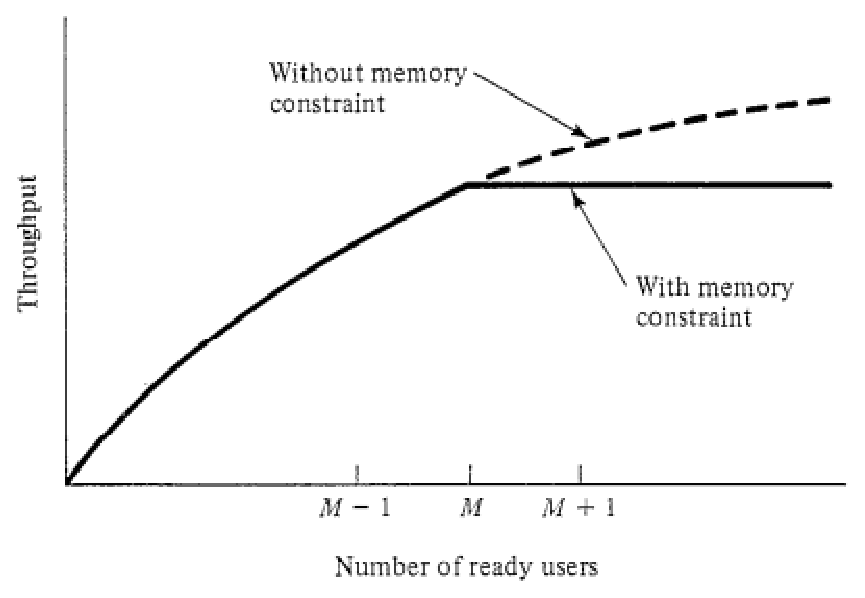
\includegraphics[width=0.62\textwidth]{image/memory-effect-on-throughput1.eps}
%  \caption{Effect of memory on throughput not considering swapping and paging.}
%  \label{fig:effect-of-memory-on-throughput} 
%\end{figure*}
%
%% In Figure \ref{fig:menory-effect}\subref{fig:effect-of-memory-on-throughput} 
%The throughput-limiting effect of a memory constraint can be even more complicated in real computer systems because of complicated memory management mechanisms such as \textit{swapping}. All current operating systems have implemented ways to oversubscribe the memory (i.e. remove the hard constraint on the number of active processes sharing memory) using a swapping mechanism. Swapping is about bringing the extra processes into memory and taking them back to a secondary larger storage as they become active. With swapping, one can highly increase the multiprogramming level with cost of frequent swapping between primary memory and secondary storage. The amount of swapping at each given time depends on  the total number of active processes $N$, and the portion of these processes that can fit into the actual memory simultaneously $M$. If $N$ is less than $M$ then no swapping will occur, otherwise there will be  swapping with some probability which depends on $M$ and $N$ (with growth of $N$ compared to $M$ the probability will be increased).
%As a result in a swapped system, when simultaneous processes are increased, lower memory leads to more overhead and placing extra demands on the I/O subsystem and the CPU.
%In an extreme case, overhead of too much swapping might take all processing resources.
%See Figure \ref{fig:throughput-multiprogramming}, adopted from \cite{lazowska_quantitative_1984}, for the effect of multiprogramming on throughput.
%
%\begin{figure*}[h]
% \centering    
%  %  \includegraphics[width=0.62\textwidth]{image/throughput-multiprogramming1.eps} 
%  \caption{Effect of multiprogramming on throughput.}
% \label{fig:throughput-multiprogramming}
%\end{figure*}
%
%% 
%% \begin{figure}[h]
%%  \centering    
%%     \subfloat[][]{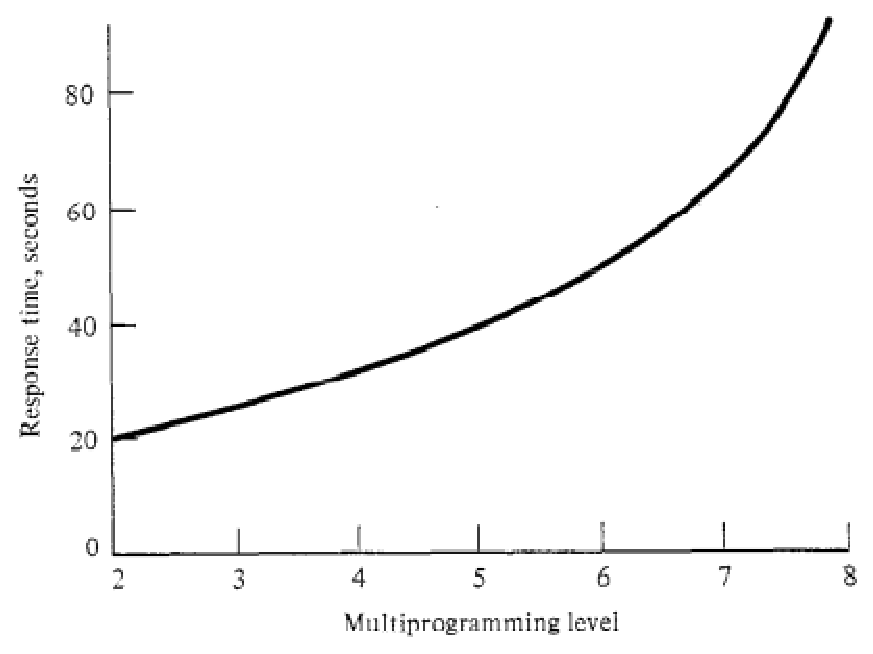
\includegraphics[width=0.42\textwidth]{image/responsetime-multiprogrammming.eps} \label{fig:responsetime-multiprogramming}}
%% %     \qquad
%%   %  \subfloat[][]{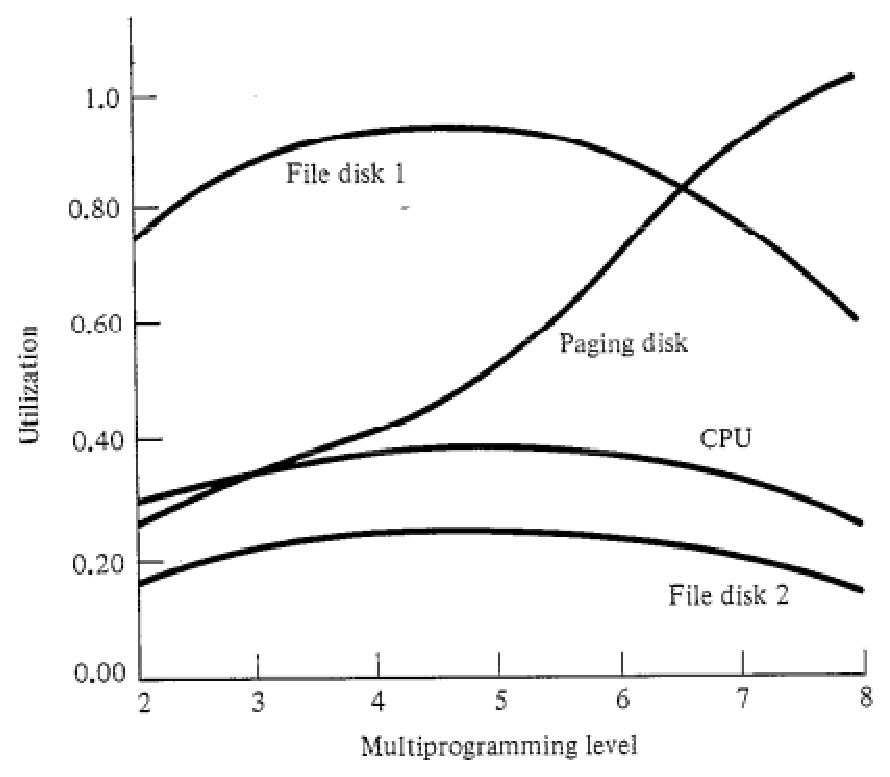
\includegraphics[width=0.42\textwidth]{image/utilization-multiprogramming.eps}\label{fig:utilization-multiprogramming}}
%%      \subfloat[][]{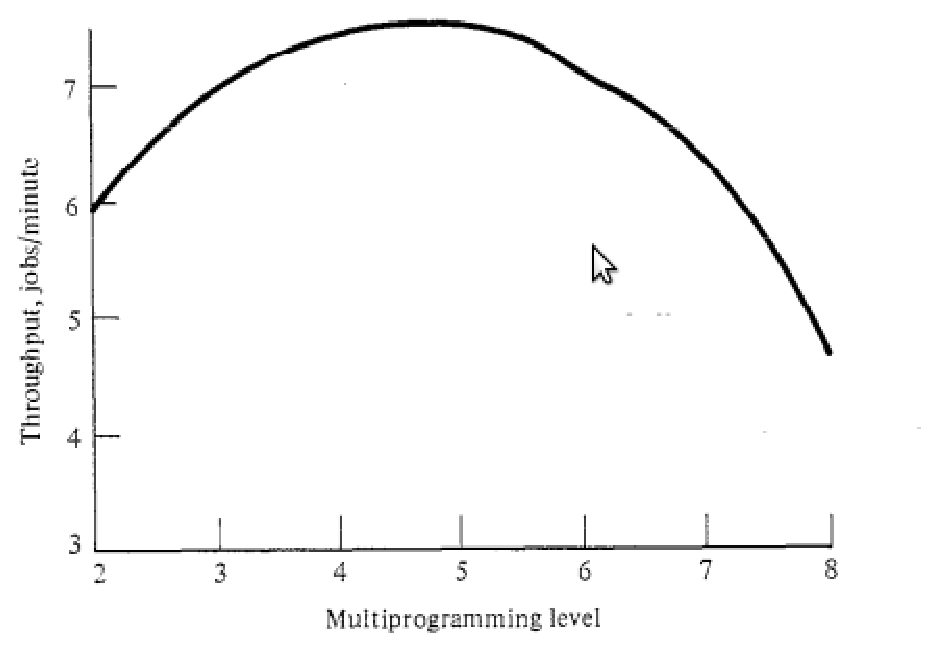
\includegraphics[width=0.42\textwidth]{image/throughput-multiprogramming.eps} \label{fig:throughput-multiprogramming}}
%%  \caption{effect multiprogramming on (a) response time (b) utilization, and (c) throughput.}
%%  \label{fig:menory-effect}
%% \end{figure}
%
%Another mechanism commonly used in current operating systems that makes it difficult to identify or predict their behavior is \textit{paging}. %contributes to efficient
%In paging, physical memory to be divided into some number of fixed-size page frames, and portions of program quantified with these fixed size pages (as opposed to the whole code or data segments) are swapped into the memory. 
%These portions are selected according to the concept of 'locality of reference': from a large address space owned by a program, only a small portion will be referenced during any short time interval.   
%Paging lets OS to allocate a much larger virtual address space for the program than the actual physical primary memory available.
%This leads to 1) accommodation of programs whose virtual address spaces are larger than the amount of physical memory
%and 2) increasing the number of concurrently active programs. 
%However, management of the virtual memory (i.e. moving pages between primary memory and disk in response to page faults) consumes CPU and I/O resources.
%
%The OS itself tries to optimize the performance of given programs % (which to CPU its internals are back box)
%for the specific amount of memory given by %to the system (from higher level management layer) by 
%(i) controlling the amount of programs that are allowed to compete for memory resources (multiprogramming level),
%(ii) distributing proper number of page frames to each of these programs, 
%(iii) choosing the pages that should occupy the page frames allocated to a program 
%and (iv) deciding on the page that should be removed from primary memory for bringing a currently non-resident referenced page.
%These items form the page replacement policy of operating system, which in conjunction with memory reference characteristics of programs
%\footnote{Reference characteristics of a program can be denoted by its \textit{lifetime function}, which is the average number of milliseconds of CPU service that elapse between page faults for various numbers of allocated page frames.},
%and the amount of given memory will result in specific system performance. 
%
%As we move up the layers of software stack tracing the effects of different configurations on memory management becomes significantly more difficult. 
%For example in container level, by modifying internal multiprogramming level of a container process (see subsection \ref{sec:modeling-thread-pools})
%its memory usage pattern (or program lifetime function) will change, resulting in different system's paging and swapping for its OS process. 
%%This forms an effective tool in controlling the overhead associated with paging and in deciding on the efficient amount of memory assigned to a VM. 
%
%
%% \begin{figure}[h]
%%  \centering
%%  
%%  % utilization-multiprogramming.eps: 0x0 pixel, 300dpi, 0.00x0.00 cm, bb=439 340 850 697
%%  \caption{.}
%%  \label{fig:utilization-multiprogramming}
%% \end{figure}
%% 
%% \begin{figure}[h]
%%  \centering
%%  
%%  % throughput-multiprogramming.eps: 0x0 pixel, 300dpi, 0.00x0.00 cm, bb=415 375 849 671
%%  \caption{Throughput versus multiprogramming.}
%%  \label{fig:throughput-multiprogramming}
%% \end{figure}
%
%\subsubsection{Modeling Tiered Software with Synchronous Calls}
%Distributed applications usually contain one or more layers of software servers. Examples include three tier database driven applications; applications developed using Java's remote method invocation (RMI), Remote Procedure Call (RPC), or Enterprise Java Beans (EJB). In such systems Performance features (e.g. response time) are affected by the software design (e.g. message passing versus synchronous calls), the multi-threading level, number of instances of software processes, and the allocation of processes to processors. The standard model for representing these systems is Layered Queuing Model (LQM) that has been developed together with its analytical techniques such as Method of Layers (MOL) \cite{rolia_method_1995}. 
%This analytical technique models the system tiers each with its own software and hardware layers and captures the contention delays at each layer or tier. Each layer is represented by a Queuing Network Model (QNMs) which can be solved by the mean value analysis (MVA). By iterating among the layers of QNMs, a fix point solution is found for the whole LQM \cite{petriu_approximate_1991}.  
%
%These models help capturing different types of resource demands at different tiers. For example, in a web based tiered system front-end servers are more stressed on their IO and CPU capabilities, I/O for direct content serving to the users, and CPU because of the connection rate and number of concurrent connections. Application servers are more CPU-stressed because of support for business logic. Finally, the requests translated by application layer to database commands are executed in backend database servers that put a lot of demand on storage tier.
% Model inputs for LQMs include: 
%(i) the structure of the model including the services and their interactions for representative scenarios, and a topology of the underlying middleware and hardware, and 
%(ii) the same set of quantitative performance metrics as flat queuing models (e.g. workload component, and service times or demands ($D_c$) for each class of service $c$ on each resource $k$). 
%% Outputs of LQM include response times ($R_c$), throughput ($X_c$) for each class and server utilization ($U_j$) for each server.
%Figure \ref{fig:lqm-of-web-application} shows a typical Layered Queuing Model (LQM) of a web-based application. We assume that there are $C$ classes of requests; the ``User'' block in the figure represents $N_c$ users in class $c$ at their browsers. $Z_c$ is used to denote the mean think time of class $c$ users. $N_c$ and $Z_c$ are the workload parameters for class $c$. 
%
%\begin{figure}[h]
%	\centering		
%%	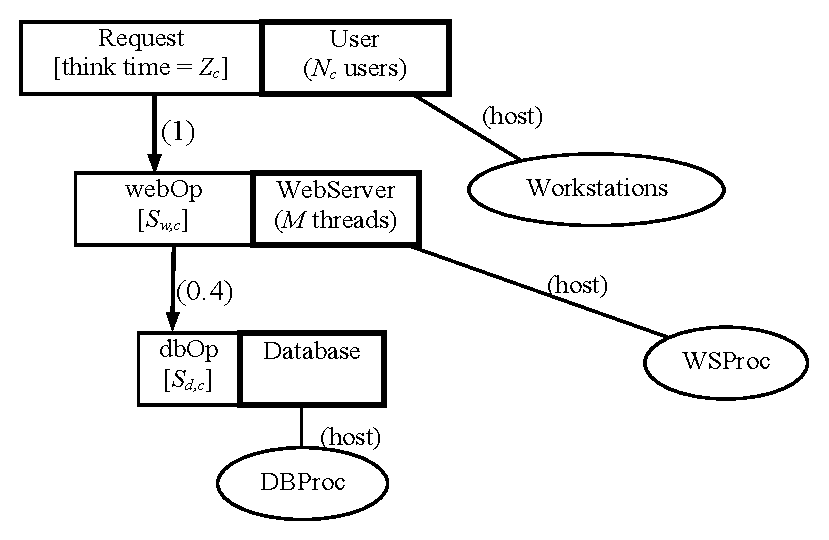
\includegraphics[width=0.45\textwidth]{image/image-LQM-structure.eps} 
%	\caption{Multiclass Layered Queuing Model of a Web application.} 
%	\label{fig:lqm-of-web-application}
%\end{figure}
%% Variation in load arriving at the system can be modeled by variations in $Z_c$ or in $N_c$; a larger $N_c$ or a smaller $Z_c$ leads to a higher level of offered load.
%The \textit{WebServer} block represents the server software with $M$ threads, running on processor \textit{WSProc} (this is indicated by the \textit{host} relationship). The box labeled \textit{webOp} represents the operation done for the users, and requires a mean CPU demand of $D_{w,c}$ for requests in class $c$ and on average one database operations. The database is running on its own device \textit{DBProc}. \textit{dbOp} represents the mean CPU demands of $D_{d,c}$ at \textit{DBProc} for a class $c$ request.
%
%Outputs of LQM of Figure \ref{fig:lqm-of-web-application} include
%mean response times to class $c$ users $\langle R_1 \dots R_C\ \rangle$, 
%mean response times to class $c$ users at database server $\langle R^d_1 \dots R^d_C \rangle$,  
%throughput of each class $c$ users $\langle X_1 \dots X_C \rangle$, 
%utilization of web server processor $U_w$, and database processor $U_d$. 


% \chapter{Estimation} 
%however the major concern is the ability to Understand the current state of the system
% since many  parameters are not observable however since they're part of the model in order to project the system state to the future we need them
% update and synchronize the model based on observed behavior of the system.
 
% \subsection{ Performance Models and Estimators} 
%Multi-class Layered Queuing Models for Services
%In this subsection we introduce Layered Queuing Model (LQM) as a model to capture the behavior of multi-tier web services deployed in a data center environment. A way to look at a web application is through the software layers introduced by the different tiers: web and application servers, and enterprise database servers; and through the hardware layer of the underlying infrastructure. LQM has been shown to be effective in modeling such software and hardware layers and in capturing the contention delays at each layer [21]. Each layer is represented by a Queuing Network Model (QNM) which can be solved by the mean value analysis. By iterating among the layers of QNMs, a fix point solution is found for the whole LQM [22].
%Model inputs for LQMs include the structure of the model, and the quantitative data capturing essential performance metrics. The structure will include the services and their interactions (called visits) for representative scenarios (or classes), a workload component with the number of users and the mean think time for each class (alternatively, the per class request arrival rates), and eventually a topology of the underlying middleware and hardware. 
%To complete the application scenarios, service times or demands for each class of service are needed. Measuring such service demands, even if technologically possible, is not practical because of the overhead introduced. In our investigation, demand metrics are instead estimated by an estimator such as the Kalman filter. Metrics that can be obtained easily by system measurement, e.g., response times, throughput and server utilization, are used to periodically calibrate the model.
%In LQM, a service is either a pure server, which executes operations on command or a more complex logical bundle of operations, which include the use of lower layer services. Such a bundle of operations may be treated as a software server. Software servers are implemented by containers, virtual machines or OS processes within virtual machines. The threads are servers to the common-queue, and the �visits� take the form of service calls (remote procedure calls, remote method invocations, messages or the semantic equivalent), and the classes of service represent methods or group of methods.
%The execution of a server (or thread) is assumed to be carried out by a single processor, or multiprocessor, called it a host or node. Execution is typically accomplished by a sequence of requests for service to the host and to other servers, and the essence of layered modeling is to capture this nesting of requests. Each request requires queuing at its corresponding server, followed by execution of a service at that server.
%Implementation of LQM modelers and solvers include LQN Solver and Apera [23].

%\singlespace
%
%\bibliographystyle{IEEEtran}
%\bibliography{mybib}
%\printindex
%
%\end{document}

